\documentclass[12pt,oneside,openany,spanish,oldfontcommands]{memoir}

% ============================================================
% CONTROL DE PÁGINAS Y SALTOS EN MEMOIR (SIN PÁGINAS EN BLANCO)
% ============================================================
\openany
\let\cleardoublepage\clearpage

% ============================================================
% IDIOMA Y TIPOGRAFÍA
% ============================================================
\usepackage[T1]{fontenc}
\usepackage[utf8]{inputenc}
\usepackage[spanish]{babel}
\usepackage{csquotes}
\usepackage{mathpazo}

% ============================================================
% BIBLIOGRAFÍA
% ============================================================
\usepackage[
  backend=biber,
  style=apa,
  sorting=nyt
]{biblatex}
\addbibresource{referencias.bib}
\DeclareLanguageMapping{spanish}{spanish-apa}

\setcounter{secnumdepth}{3}
\setcounter{tocdepth}{3}

% Formato general
\setlength{\parskip}{\medskipamount}
\setlength{\parindent}{0pt}

% ============================================================
% MATEMÁTICAS, ALGORITMOS Y CÓDIGO
% ============================================================
\usepackage{amsmath}
\usepackage{amssymb}
\usepackage{dsfont}

\usepackage{algorithm}
\usepackage{algorithmicx}
\usepackage{algpseudocode}

\algdef{SE}[VARIABLES]{VARIABLES}{EndVariables}
  {\algorithmicvariables}
  {\algorithmicend\ \algorithmicvariables}
\algnewcommand{\algorithmicvariables}{\textbf{variables globales}}

\newcommand{\Tau}{\mathrm{T}}
\newcommand{\I}{\mathds{1}}

\usepackage{listings}
\renewcommand{\lstlistingname}{Listado de código}

% ============================================================
% FIGURAS Y TABLAS
% ============================================================
\usepackage{graphicx}
\graphicspath{{./}{../diagramas/}{docs/diagramas/}{images/}}

\usepackage{booktabs}
\usepackage{array}
\usepackage{longtable}
\usepackage{tabularx}
\usepackage{multirow}
\usepackage{makecell}
\usepackage{adjustbox}
\usepackage{pdflscape}
\usepackage{float}
\usepackage{placeins}
\usepackage[table]{xcolor}
\usepackage{caption}

\captionsetup{
  font=small,
  labelfont=bf,
  labelsep=colon
}

\renewcommand{\arraystretch}{1.15}

% Colores institucionales y del proyecto
\definecolor{uctblue}{HTML}{1B2A4B}
\definecolor{uctlight}{HTML}{D9E6F5}
\definecolor{ganttblue}{HTML}{1A659E}
\definecolor{ganttlight}{HTML}{A7D2ED}

% ============================================================
% UTILIDADES
% ============================================================
\usepackage{url}
\usepackage[none]{hyphenat}
\usepackage{fancyvrb}
\usepackage{alltt}

\DefineVerbatimEnvironment{example}{Verbatim}{fontsize=\scriptsize}
\renewenvironment{example*}{\begin{alltt}}{\end{alltt}}

\DefineVerbatimEnvironment{Sinput}{Verbatim}{}
\DefineVerbatimEnvironment{Soutput}{Verbatim}{}
\DefineVerbatimEnvironment{Scode}{Verbatim}{}
\DefineVerbatimEnvironment{Sin}{Verbatim}{}
\DefineVerbatimEnvironment{Sout}{Verbatim}{}
\newenvironment{Schunk}{}{}

% ============================================================
% HIPERVÍNCULOS
% ============================================================
\usepackage[
  colorlinks=true,
  linkcolor=uctblue,
  citecolor=uctblue,
  urlcolor=uctblue
]{hyperref}

% ============================================================
% FORMATO DE CAPÍTULOS Y SECCIONES (COMPACTO Y EN UNA SOLA LÍNEA)
% ============================================================
\makechapterstyle{compacto}{%
  \setlength{\beforechapskip}{0pt}
  \setlength{\midchapskip}{0pt}
  \setlength{\afterchapskip}{14pt}
  \renewcommand*{\chapterheadstart}{\vspace*{0pt}}
  \renewcommand*{\printchaptername}{}
  \renewcommand*{\chapternamenum}{}
  \renewcommand*{\chapnumfont}{\normalfont\LARGE\bfseries}
  \renewcommand*{\chaptitlefont}{\normalfont\LARGE\bfseries}
  \renewcommand*{\printchapternum}{\chapnumfont\thechapter.\space}
  \renewcommand*{\afterchapternum}{}
  \renewcommand*{\printchaptertitle}[1]{\chaptitlefont ##1}
  \renewcommand*{\afterchaptertitle}{\par\nobreak\vskip \afterchapskip}
}
\chapterstyle{compacto}

% Ajuste proporcional de secciones y subsecciones
\setsecheadstyle{\normalfont\Large\bfseries}
\setsubsecheadstyle{\normalfont\large\bfseries}
\setsubsubsecheadstyle{\normalfont\normalsize\bfseries}

% ============================================================
% COMANDO SEGURO PARA LOGO INSTITUCIONAL (OVERLEAF / REPO)
% ============================================================
\newcommand{\insertLogoHeader}{%
  \IfFileExists{logo.png}{%
    \includegraphics[height=27pt]{logo.png}%
  }{%
    \IfFileExists{Logo_depto_ing_informatica.png}{%
      \includegraphics[height=27pt]{Logo_depto_ing_informatica.png}%
    }{%
      \scriptsize Logo UCT%
    }%
  }%
}

\newcommand{\insertLogoCover}[1]{%
  \IfFileExists{logo.png}{%
    \includegraphics[width=#1]{logo.png}%
  }{%
    \IfFileExists{Logo_depto_ing_informatica.png}{%
      \includegraphics[width=#1]{Logo_depto_ing_informatica.png}%
    }{%
      \fbox{\parbox[c][2.0cm][c]{0.90\textwidth}{\centering
      \textbf{LOGO INSTITUCIONAL -- incorporar logo.png}}}%
    }%
  }%
}

% ============================================================
% ENCABEZADO Y PIE DE PÁGINA
% ============================================================
\usepackage{fancyhdr}

\setlength{\headheight}{38pt}
\setlength{\headsep}{12pt}

\fancypagestyle{mainstyle}{%
  \fancyhf{}
  \renewcommand{\headrulewidth}{0.3pt}
  \renewcommand{\footrulewidth}{0pt}

  \fancyhead[L]{\insertLogoHeader}

  \fancyhead[R]{%
    \small
    \color{uctblue}
    Trabajo de Título INFO-1197\\
    \textit{Red LoRaWAN UCT -- Etapa 3}
  }

  \fancyfoot[C]{\small\thepage}
}

\fancypagestyle{plain}{%
  \fancyhf{}
  \renewcommand{\headrulewidth}{0.3pt}
  \renewcommand{\footrulewidth}{0pt}

  \fancyhead[L]{\insertLogoHeader}

  \fancyhead[R]{%
    \small
    \color{uctblue}
    Trabajo de Título INFO-1197\\
    \textit{Red LoRaWAN UCT -- Etapa 3}
  }

  \fancyfoot[C]{\small\thepage}
}

\pagestyle{mainstyle}

% ============================================================
% TÍTULOS DE ÍNDICES
% ============================================================
\renewcommand{\printtoctitle}[1]{\chaptitlefont #1}
\renewcommand{\printloftitle}[1]{\chaptitlefont #1}
\renewcommand{\printlottitle}[1]{\chaptitlefont #1}

% ============================================================
% COMANDOS AUXILIARES
% ============================================================
\newcommand{\tituloTesis}{%
  Diseño, implementación y evaluación del rendimiento de una red LoRaWAN
  para la sensorización del Campus Dr. Luis Rivas del Canto%
}

\begin{document}
\sloppy

% ============================================================
% PORTADA
% ============================================================
\thispagestyle{empty}
\pagenumbering{gobble}

\vspace*{-6\baselineskip}

\begin{center}
  \insertLogoCover{\textwidth}
\end{center}

\vspace{3.0cm}

\begin{center}
  \textbf{\tituloTesis}
\end{center}

\vspace{3.5cm}

\begin{center}
  por
\end{center}

\vspace{0.4cm}

\begin{center}
  Eduardo Remigio Mariqueo Porma
\end{center}

\vspace{3.0cm}

\begin{center}
  Trabajo de Título presentado a la\\
  Facultad de Ingeniería de la Universidad Católica de Temuco\\
  Para Optar al Título de Ingeniero Civil Informático.
\end{center}

\vfill

\begin{center}
  -- Temuco, Noviembre 2026 --
\end{center}

% ============================================================
% COMISIÓN EXAMEN DE TÍTULO
% ============================================================
\clearpage
\thispagestyle{empty}

\begin{center}
  \vspace*{-9\baselineskip}
  \insertLogoCover{0.8\textwidth}
  \par
  \textbf{COMISIÓN EXAMEN DE TÍTULO}
\end{center}

Este Examen de Título ha sido realizado en la Escuela de Ingeniería Informática:

\vspace{0.4cm}

\begin{tabular}{>{\raggedright\arraybackslash}p{0.38\textwidth}>{\centering\arraybackslash}p{0.48\textwidth}}
Presidente Comisión: &
\dotfill\\
& \textbf{Por designar}\\
& Escuela de Ingeniería Informática\\[0.8cm]

Profesor Guía: &
\dotfill\\
& \textbf{Prof. Mario Villanueva}\\
& Profesor Guía\\
& Escuela de Ingeniería Informática\\[0.8cm]

Profesor Informante: &
\dotfill\\
& \textbf{Por designar}\\
& Escuela de Ingeniería Informática\\[0.8cm]

Jefe de Carrera de Ingeniería Civil Informática: &
\dotfill\\
& \textbf{Prof. Mario Villanueva}\\
& Magíster en Gestión de Tecnologías de la Información\\
& Ingeniero Informático\\
& Jefe de Carrera Ing. Civil Informática
\end{tabular}

\vfill
Temuco, Noviembre 2026.

% ============================================================
% INFORME PROFESOR GUÍA
% ============================================================
\clearpage
\thispagestyle{empty}

\begin{center}
  \vspace*{-9\baselineskip}
  \insertLogoCover{0.8\textwidth}
  \par
  \textbf{INFORME TRABAJO DE TÍTULO}
\end{center}

\vspace{1cm}

\begin{tabular}{>{\raggedright\arraybackslash}p{0.20\textwidth}>{\raggedright\arraybackslash}p{0.02\textwidth}>{\raggedright\arraybackslash}p{0.70\textwidth}}
TÍTULO & : & ``\tituloTesis''\\
& & \\
ALUMNO & : & Eduardo Mariqueo
\end{tabular}

\vspace{1cm}

En mi calidad de Profesor Guía, mis apreciaciones del presente informe de Trabajo de Título
son las siguientes:

\begin{itemize}
  \item Apreciación 1.
  \item Apreciación 2.
  \item Apreciación 3.
\end{itemize}

De acuerdo con estas consideraciones califico el desarrollo de este Trabajo de Título con
\textbf{nota X,X (nota en letras).}

\vspace{1cm}

\begin{flushright}
\rule{65mm}{0.2mm}\\
\textbf{Prof. Mario Villanueva}\\
\textbf{Profesor Guía}
\end{flushright}

\vspace{1cm}

Temuco, Noviembre 2026.

% ============================================================
% INFORME PROFESOR INFORMANTE
% ============================================================
\clearpage
\thispagestyle{empty}

\begin{center}
  \vspace*{-9\baselineskip}
  \insertLogoCover{0.8\textwidth}
  \par
  \textbf{INFORME TRABAJO DE TÍTULO}
\end{center}

\vspace{0.8cm}

\begin{tabular}{>{\raggedright\arraybackslash}p{0.20\textwidth}>{\raggedright\arraybackslash}p{0.02\textwidth}>{\raggedright\arraybackslash}p{0.70\textwidth}}
TÍTULO & : & ``\tituloTesis''\\
& & \\
ALUMNO & : & Eduardo Mariqueo
\end{tabular}

\vspace{1cm}

En mi calidad de Profesor Informante, mis apreciaciones del presente informe de Trabajo de
Título son las siguientes:

\begin{itemize}
  \item Apreciación 1.
  \item Apreciación 2.
  \item Apreciación 3.
\end{itemize}

De acuerdo con estas consideraciones califico el desarrollo de este Trabajo de Título con
\textbf{nota X,X (nota en letras).}

\vspace{1cm}

\begin{flushright}
\rule{65mm}{0.2mm}\\
\textbf{Por designar}\\
\textbf{Profesor Informante}
\end{flushright}

\vspace{1cm}

Temuco, Noviembre 2026.

% ============================================================
% AGRADECIMIENTOS
% ============================================================
\clearpage
\thispagestyle{empty}

\begin{center}
  \textbf{AGRADECIMIENTOS}
\end{center}

\vspace{1cm}

Agradezco a mi profesor guía y Jefe de Carrera, Prof. Mario Villanueva, por su orientación,
disposición y acompañamiento presencial durante el desarrollo e implementación de este Trabajo
de Título. Agradezco también a la Universidad Católica de Temuco y a la Escuela de Ingeniería
Informática por facilitar el acceso a la infraestructura y al equipamiento de telecomunicaciones
necesarios para materializar el prototipo. Finalmente, agradezco a mi familia por su apoyo
constante a lo largo de este proceso.

\vfill

\noindent\textbf{Nota del autor:} \small Se declara que durante la redacción de este trabajo se utilizaron herramientas de inteligencia artificial exclusivamente como apoyo auxiliar para tareas de redacción y revisión lingüística, sin intervenir en el planteamiento conceptual, la metodología ni los resultados empíricos del estudio.

% ============================================================
% ÍNDICES
% ============================================================
\clearpage
\pagenumbering{roman}
\pagestyle{empty}

\tableofcontents*
\clearpage

\listoftables*
\clearpage

\listoffigures*
\clearpage

% ============================================================
% RESUMEN
% ============================================================
\thispagestyle{empty}

\begin{abstract}
\addcontentsline{toc}{chapter}{Resumen}

Este documento consolida las Etapas~1 y 2, y presenta integralmente el desarrollo de la Etapa~3 (Implementación Física, Optimización y Pruebas Preliminares) del Trabajo de Título orientado a diseñar, implementar y evaluar el rendimiento de una red LoRaWAN para la sensorización del Campus Dr. Luis Rivas del Canto de la Universidad Católica de Temuco (UCT). En el ámbito radioeléctrico, la solución opera en estricto cumplimiento de las Resoluciones Exentas N.º 1.985 de 2017 y N.º 737 de 2025 de la SUBTEL bajo el plan regional LoRaWAN AU915 Sub-banda 2 (916,8--918,2~MHz) a una potencia máxima de 14~dBm (25~mW) con activación criptográfica OTAA (AES-128).

Durante la Etapa~3 se optimizó la arquitectura de red incorporando un Gateway semi-industrial Milesight UG65 como concentrador controlador con servidor de red embebido (\textit{Embedded Network Server}), articulado en topología de flota (\textit{Gateway Fleet}) junto al Gateway Milesight UG63 como agente secundario mediante MQTT interno (puerto 18883). Esta decisión elimina dependencias de servidores externos durante la fase de prototipo, resguardando la arquitectura ChirpStack v4 documentada como alternativa de respaldo y escalamiento para futuros proyectos del Departamento de Informática. Asimismo, se estandarizó un payload binario compacto de 10~bytes en formato \textit{Big-Endian} ($\text{ToA} \approx 46,3\,\text{ms}$ en SF7/125~kHz), cuatro programas modulares en C++/Arduino IDE (Sesiones Tipo~A y Tipo~B) para nodos Heltec WiFi LoRa 32 V3 con sensórica DHT11 real, y un banco de pruebas local (\textit{testbed}) en Python/SQLite que opera como respaldo autónomo y se complementa con el Trabajo de Título paralelo orientado al sistema integrado de gestión y monitoreo IoT.

El despliegue espacial intra-campus ubica la concentración en el Edificio~10 (Facultad de Ingeniería), estableciendo distancias aproximadas homologadas hacia el Edificio~16 en línea de vista directa ($\text{LOS} \approx 80\,\text{m}$) y hacia el Edificio~08 en condición obstruida ($\text{NLOS} \approx 85\,\text{m}$, bloqueado por el Edificio~09). Las pruebas preliminares acumulan 4.824 tramas reales almacenadas ($\approx 96\,\text{bytes/trama}$), evidenciando pérdidas de paquetes entre $0,00\%$ y $2,22\%$ ($PL \le 10\%$), disponibilidad estacionaria del $100,0\%$ ($A \ge 90\%$), retardos medios de confirmación $\overline{T_{\mathrm{conf}}} \approx 1,1\text{--}1,2\,\text{s}$ ($T_{\mathrm{conf}} \le 6,0\,\text{s}$) y demodulación efectiva hasta $-105\,\text{dBm}$ ($\text{SNR} = -9,8\,\text{dB}$) en pruebas de recorrido, alcanzando un $82,9\%$ de ejecución global del backlog PPDIOO (136 de 164 horas).

\textbf{Palabras clave:} LoRaWAN, IoT, sensórica intra-campus, Milesight UG65, LPWAN, PPDIOO, propagación LOS/NLOS.
\end{abstract}

% ============================================================
% ABSTRACT
% ============================================================
\clearpage
\thispagestyle{empty}

\renewcommand{\abstractname}{Abstract}

\begin{abstract}
\addcontentsline{toc}{chapter}{Abstract}

This document consolidates Stages~1 and 2, and comprehensively presents Stage~3 (Physical Implementation, Design Optimization, and Preliminary Testing) of the Degree Project aimed at designing, implementing, and evaluating the performance of a LoRaWAN network prototype for sensorizing the Dr. Luis Rivas del Canto Campus at Universidad Católica de Temuco (UCT). Regarding spectrum regulation, the prototype strictly complies with Chilean SUBTEL Exempt Resolutions No. 1,985 (2017) and No. 737 (2025) under the LoRaWAN AU915 Sub-band 2 channel plan (916.8--918.2~MHz) at 14~dBm (25~mW) transmit power using AES-128 Over-The-Air Activation (OTAA).

During Stage~3, the network architecture was optimized by integrating a semi-industrial Milesight UG65 LoRaWAN Gateway operating its native Embedded Network Server as the primary controller for the prototype, paired in a multi-gateway fleet topology with a Milesight UG63 agent gateway via internal MQTT (port 18883). While eliminating external server single points of failure for prototype validation, the ChirpStack v4 stack remains documented as an operational backup and scalable alternative for future departmental projects. Furthermore, a deterministic 10-byte Big-Endian binary payload ($\text{ToA} \approx 46.3\,\text{ms}$ at SF7/125~kHz), four modular C++/Arduino IDE firmware sketches (Type~A unconfirmed and Type~B confirmed sessions) for Heltec WiFi LoRa 32 V3 nodes with DHT11 sensors, and a lightweight Python/SQLite local laboratory testbed were implemented, explicitly delineating its scope as a validation bench complementary to a parallel thesis focused on an enterprise IoT device management and monitoring platform.

The spatial campus deployment places the gateway infrastructure in Building~10 (Faculty of Engineering), establishing equalized approximate link distances toward Building~16 under direct Line-of-Sight ($\text{LOS} \approx 80\,\text{m}$) and Building~08 under Non-Line-of-Sight ($\text{NLOS} \approx 85\,\text{m}$, obstructed by Building~09). Preliminary empirical campaigns collected 4,824 real frames ($\approx 96\,\text{bytes/record}$), demonstrating packet loss rates between $0.00\%$ and $2.22\%$ ($PL \le 10\%$), $100.0\%$ stationary link availability ($A \ge 90\%$), mean confirmation delays of $\overline{T_{\mathrm{conf}}} \approx 1.1\text{--}1.2\,\text{s}$ ($T_{\mathrm{conf}} \le 6.0\,\text{s}$), and sub-noise CSS demodulation down to $-105\,\text{dBm}$ ($\text{SNR} = -9.8\,\text{dB}$) during walk-tests, achieving $82.9\%$ overall completion of the PPDIOO project backlog (136 of 164 hours).

\textbf{Keywords:} LoRaWAN, IoT, campus sensing, Milesight UG65, LPWAN, PPDIOO, LOS/NLOS propagation.
\end{abstract}

% ============================================================
% CONTENIDO PRINCIPAL
% ============================================================
\clearpage
\pagenumbering{arabic}
\setcounter{page}{1}
\pagestyle{mainstyle}

% ============================================================
% CAPÍTULO 1: INTRODUCCIÓN
% ============================================================
\chapter{Introducción}

\section{Contexto general}

El proyecto aborda la necesidad de contar con una red de conectividad de bajo consumo
para sensores IoT dentro del Campus Dr. Luis Rivas del Canto (Facultad de Ingeniería) de
la Universidad Católica de Temuco. A diferencia de una red Wi-Fi tradicional, una solución
basada en LoRaWAN permite transportar datos de sensores distribuidos en distintos
puntos del campus con menor consumo energético y sin depender necesariamente de la
cobertura inalámbrica institucional existente.

La propuesta contempla el diseño, implementación y evaluación de un prototipo de conectividad
basado en tecnología LoRaWAN, con infraestructura de concentración emplazada en la Facultad de
Ingeniería y nodos sensores desplegados en distintos edificios del campus, cuyos datos se
publican hacia la red IP mediante MQTT y se registran en un entorno de visualización y captura.
El propósito del estudio no es asumir a priori la superioridad de LoRaWAN frente a otras
tecnologías, sino establecer una base técnica, metodológica y empírica que permita cuantificar
objetivamente su desempeño en el escenario universitario real, considerando la presencia de
obstáculos estructurales propios del recinto (edificios, losas y muros de hormigón armado).

\section{Problema}

La necesidad de este proyecto se relaciona con la disponibilidad de una alternativa de
conectividad de bajo consumo y de bajo costo operativo para el transporte de datos de
sensores IoT dentro del campus. Previo a esta iniciativa, no se contaba con una infraestructura
propia de bajo consumo energético orientada específicamente a telemetría de baja tasa, lo que
limitaba el desarrollo experimental de aplicaciones de sensórica dentro de la Facultad de
Ingeniería.

Una solución de conectividad para nodos de telemetría debe responder a las demandas
reales de monitoreo intra-campus. Entre las aplicaciones concretas de sensorización
identificadas para la Facultad de Ingeniería se incluyen: (1) el monitoreo de confort
ambiental y habitabilidad (temperatura, humedad relativa y concentración de $\text{CO}_2$)
en salas de clases y laboratorios docentes de informática; (2) la telemetría en áreas verdes
y patios perimetrales del campus (humedad de suelo, luminosidad e índice de radiación); y
(3) la supervisión del estado operativo y consumos eléctricos en tableros de talleres de
especialidad. La implementación de tales iniciativas bajo la red inalámbrica convencional se ve
restringida por factores de consumo energético, limitaciones de alcance en exteriores, operación
radioeléctrica ante obstáculos estructurales (edificios, muros de hormigón armado) y la
complejidad de autenticar microcontroladores de bajo costo en redes Wi-Fi corporativas
(WPA2-Enterprise). Por ello, resulta pertinente evaluar una infraestructura LPWAN propia,
concebida específicamente para el transporte eficiente de tramas cortas de telemetría.

El problema se formula operacionalmente de la siguiente manera:

\begin{quote}
\textit{
La UCT requiere evaluar una alternativa de conectividad propia para transportar datos de
sensores IoT dentro del Campus Dr. Luis Rivas del Canto, considerando restricciones de
consumo energético, la presencia de obstáculos estructurales y la dependencia de la
infraestructura de red existente, y permitiendo la visualización y registro estructurado de
dichos datos.
}
\end{quote}

A partir de esta formulación se plantea la siguiente pregunta de investigación:

\begin{quote}
\textit{
¿En qué medida un prototipo de red LoRaWAN implementado dentro del Campus Dr. Luis Rivas
del Canto permite transportar y visualizar datos de sensores IoT de manera técnicamente
viable, considerando la presencia de obstáculos estructurales dentro del campus?
}
\end{quote}

\subsection{Limitaciones de la infraestructura de conectividad actual}
\label{sec:limitaciones-infra}

La insuficiencia de la infraestructura Wi-Fi existente para telemetría IoT de bajo consumo se
fundamenta en las siguientes restricciones estructurales y tecnológicas:

\begin{enumerate}
  \item \textbf{Incompatibilidad energética:} Los nodos IoT de telemetría de baja tasa
  están diseñados para operar con baterías durante meses o años. El estándar Wi-Fi
  (IEEE 802.11) presenta consumos energéticos del orden de centenares de miliamperios
  durante la transmisión y asociación, incompatibles con baterías compactas típicas en
  sensores autónomos \parencite{callebaut2020}. LoRaWAN, en contraste, opera en el rango
  de microamperios en reposo y decenas de miliamperios durante breves ventanas de transmisión
  ($\text{ToA} < 50\,\text{ms}$ en SF7), adecuándose a ciclos de trabajo reducidos.

  \item \textbf{Dependencia de infraestructura densa de puntos de acceso:} La red Wi-Fi
  institucional está optimizada para zonas de alta concurrencia estudiantil en interiores.
  En un campus universitario con múltiples bloques edificados, los sensores ubicados en
  entretechos, fachadas exteriores, patios o áreas verdes quedan frecuentemente fuera del
  radio útil de los puntos de acceso (AP) existentes.

  \item \textbf{Ausencia de infraestructura LPWAN departamental previa:} La Escuela de
  Ingeniería Informática no disponía de una red LPWAN (\textit{Low Power Wide Area Network})
  operativa y documentada que sirviera como plataforma base para proyectos de pregrado,
  investigación aplicada y pruebas de protocolos IoT.
\end{enumerate}

\section{Alcance y delimitaciones}

El alcance general del Trabajo de Título comprende la formulación del problema, la especificación
de requerimientos y diseño arquitectónico (Etapas~1 y 2), la implementación física de gateways,
nodos sensores, códec de carga útil y banco local de captura junto con la ejecución de pruebas
preliminares (Etapa~3), y la evaluación experimental sistemática en terreno para determinar la
viabilidad técnica de la red (Etapa~4).

Dentro de las delimitaciones metodológicas del proyecto, se establece explícitamente que:
\begin{itemize}
  \item La arquitectura de comunicaciones emplea exclusivamente \textbf{LoRaWAN estándar}
  \parencite{lorawan1_0_4} sobre el plan regional AU915 Sub-banda~2, descartándose enlaces LoRa
  propietarios punto a punto (P2P) a fin de garantizar compatibilidad nativa con concentradores
  multicanal basados en Semtech SX1302.
  \item El foco científico y de ingeniería del presente trabajo reside en la \textbf{capa física
  de radiofrecuencia, capa MAC LoRaWAN, propagación LOS/NLOS y métricas de calidad de servicio
  (QoS)}. En consecuencia, el dashboard web implementado en este repositorio cumple estrictamente
  el rol de \textbf{banco de pruebas de laboratorio (\textit{testbed}) y respaldo operativo local},
  articulándose de forma complementaria con el Trabajo de Título desarrollado paralelamente por el
  estudiante Vicente Ramírez (\textit{``Sistema integrado para el registro, gestión y monitoreo de
  dispositivos IoT''}), encargado de la capa de aplicación empresarial, gestión avanzada de
  dispositivos y seguridad en producción.
\end{itemize}

\section{Estado del arte}

El estado del arte sustenta la selección tecnológica y los umbrales de rendimiento mediante
estudios empíricos previos sobre LoRa/LoRaWAN, telemetría IoT y propagación radioeléctrica en
recintos construidos \parencite{rademacher2021,callebaut2020,bianco2021,ahmed2024vegetacion}.

En particular, \textcite{rademacher2021} reportan una campaña de medición a gran escala
(más de 112.000 muestras) en un área urbana de 200~km\textsuperscript{2}, comparando once
modelos de pérdida de trayectoria y concluyendo que el modelo log-distancia ofrece estimaciones
consistentes frente a modelos deterministas complejos. Por su parte, \textcite{callebaut2020}
caracterizan enlaces LoRa en entornos urbano, forestal y costero, evidenciando que la baja altura
de antena incrementa severamente la pérdida de trayectoria. El trabajo de \textcite{bianco2021}
examina la propagación LoRa bajo obstrucción topográfica severa, mientras que
\textcite{ahmed2024vegetacion} cuantifican la degradación de la tasa de entrega de paquetes (PDR)
y de la relación señal-ruido (SNR) ante follaje y obstáculos físicos.

En escenarios directamente comparables de campus universitarios, \textcite{kaur2024campus}
analizan experimentalmente una red LoRa de bajo ciclo de trabajo en Amity University (India) bajo
condiciones \textit{indoor} y \textit{outdoor}, reportando tasas de entrega $\text{PDR} \geq 90\%$
en línea de vista y caídas pronunciadas al atravesar muros estructurales. De modo complementario,
\textcite{barrachina2023campus} despliegan y evalúan una red LoRaWAN multi-gateway en la
Universitat Autònoma de Barcelona (UAB), demostrando que la densificación mediante más de un
concentrador mitiga eficazmente las zonas de sombra (\textit{shadowing}) generadas por edificios
universitarios de hormigón.

\subsection{Síntesis de trabajos relacionados}

En el Cuadro~\ref{tab:estado-arte} se sintetizan las investigaciones de referencia que sustentan
el diseño experimental del proyecto.

\begin{table}[H]
\centering
\caption{Síntesis del estado del arte}
\label{tab:estado-arte}
\scriptsize
\begin{tabularx}{\textwidth}{p{2.5cm} X X X}
\toprule
\textbf{Referencia} & \textbf{Problema} & \textbf{Enfoque} & \textbf{Aporte al proyecto}\\
\midrule
\textcite{rademacher2021}
&
Predicción de cobertura en redes LoRa urbanas mediante modelos de pérdida de trayectoria.
&
Campaña de medición a gran escala (230 días, $>$112.000 muestras) y comparación de 11 modelos empíricos.
&
Sustenta el uso del modelo log-distancia con \textit{shadowing} como línea base analítica intra-campus.
\\
\midrule
\textcite{callebaut2020}
&
Caracterización de enlaces LoRa en distintos entornos físicos.
&
Campañas de medición en entorno urbano, forestal y costero; modelamiento con datos censurados.
&
Demuestra el impacto de la altura de antena y sustenta la ventaja energética frente a IEEE 802.11.
\\
\midrule
\textcite{bianco2021}
&
Comunicación LoRa en condiciones de obstrucción severa.
&
Mediciones empíricas de pérdida de trayectoria bajo bloqueo estructural y topográfico.
&
Aporta criterios de margen de enlace aplicables a la condición NLOS entre edificios del campus.
\\
\midrule
\textcite{ahmed2024vegetacion}
&
Efecto de obstáculos físicos y vegetación sobre enlaces LoRa.
&
Evaluación de PDR, RSSI y SNR en función de distancia, obstrucción y factor de dispersión (SF).
&
Justifica el umbral de pérdida aceptable ($PL \leq 10\%$) en telemetría ambiental de baja tasa.
\\
\midrule
\textcite{kaur2024campus}
&
Rendimiento de red IoT LoRa de bajo ciclo de trabajo en campus universitario.
&
Análisis experimental \textit{indoor/outdoor} en Amity University variando SF y tasa de codificación.
&
Referente directo en campus construido: confirma $\text{PDR} \geq 90\%$ en LOS y atenuación por muros.
\\
\midrule
\textcite{barrachina2023campus}
&
Despliegue y análisis de red LoRaWAN multi-gateway en recinto universitario.
&
Simulación radioeléctrica y campañas empíricas en la UAB para mitigar zonas de sombra.
&
Sustenta la topología multi-gateway (flota UG65 + UG63) y el umbral de disponibilidad $A \geq 90\%$.
\\
\bottomrule
\end{tabularx}
\end{table}

\section{Objetivos}

\subsection{Objetivo general}

Diseñar, implementar y evaluar el rendimiento de un prototipo de red LoRaWAN para la
sensorización del Campus Dr. Luis Rivas del Canto de la UCT, determinando su viabilidad
técnica mediante pruebas controladas de funcionamiento y rendimiento.

\subsection{Objetivos específicos}

\begin{enumerate}
  \item \textbf{O1.} Desplegar la infraestructura física del prototipo, compuesta por
  concentración LoRaWAN ubicada en la Facultad de Ingeniería y al menos dos nodos sensores Heltec
  WiFi LoRa 32 V3 en distintos puntos del Campus Dr. Luis Rivas del Canto, verificando su
  instalación y funcionamiento operativo.

  \item \textbf{O2.} Integrar la infraestructura Gateway LoRaWAN con el entorno de red IP definido
  para el prototipo, verificando que las tramas correctamente demoduladas y decodificadas sean
  publicadas vía MQTT y entregadas íntegras al destino de registro.

  \item \textbf{O3.} Implementar un dashboard de visualización y captura de laboratorio que
  consuma las tramas publicadas vía MQTT y presente el identificador del nodo sensor, la marca
  temporal, las variables ambientales medidas y las métricas de radiofrecuencia (RSSI y SNR).

  \item \textbf{O4.} Evaluar el rendimiento de la red desplegada dentro del campus mediante
  sesiones de tráfico controlado de 100 tramas por nodo (Sesiones Tipo~A, tramas no confirmadas,
  $NbTrans = 1$) en condiciones LOS y NLOS, complementadas con sesiones de tramas confirmadas para
  la medición de retardo (Sesiones Tipo~B, $\geq 30$ tramas confirmadas por sesión). La red se
  considerará \textbf{técnicamente viable} si cumple simultáneamente los siguientes umbrales SMART:
  \begin{itemize}
    \item \textbf{Pérdida de paquetes:} $PL \leq 10\%$ ($\text{PDR} \geq 90\%$)
    \parencite{kaur2024campus,ahmed2024vegetacion};
    \item \textbf{Retardo de confirmación:} $T_{\mathrm{conf}} \leq 6,0\,\text{s}$, consistente
    con las ventanas RX1 ($1\,\text{s}$) y RX2 ($2\,\text{s}$) de LoRaWAN Clase~A
    \parencite{lorawan1_0_4};
    \item \textbf{Disponibilidad:} $A \geq 90\%$ en operación estacionaria
    \parencite{barrachina2023campus}.
  \end{itemize}
\end{enumerate}

\subsection{Criterios SMART}

\begin{table}[H]
\centering
\caption{Objetivos específicos y criterios SMART}
\label{tab:smart}
\tiny
\setlength{\tabcolsep}{3pt}
\renewcommand{\arraystretch}{1.25}
\begin{tabularx}{\textwidth}{
  >{\bfseries\centering\arraybackslash}p{0.5cm}
  >{\raggedright\arraybackslash}p{2.0cm}
  >{\raggedright\arraybackslash\hsize=1.05\hsize}X
  >{\raggedright\arraybackslash\hsize=1.05\hsize}X
  >{\raggedright\arraybackslash\hsize=0.95\hsize}X
  >{\raggedright\arraybackslash\hsize=0.95\hsize}X
  >{\raggedright\arraybackslash\hsize=1.00\hsize}X}
\toprule
\textbf{ID} &
\textbf{Objetivo} &
\textbf{S: específico} &
\textbf{M: medible} &
\textbf{A: alcanzable} &
\textbf{R: relevante} &
\textbf{T: temporizado}\\
\midrule
O1 &
Desplegar la infraestructura física del prototipo. &
Infraestructura Gateway LoRaWAN en Facultad de Ingeniería y al menos 2 nodos sensores en el campus. &
Instalación operativa de concentradores y nodos con enlace OTAA verificado. &
Hardware institucional provisto por el Departamento de Informática. &
Construye la planta física requerida para la evaluación experimental. &
Septiembre--Octubre 2026 (Etapas~2 y 3).\\
\midrule
O2 &
Integrar el Gateway con el entorno IP de prueba. &
Decodificar y publicar hacia la red IP las tramas recibidas mediante MQTT. &
Trazabilidad 1:1 entre tramas demoduladas y mensajes JSON publicados en el broker. &
Integración directa sobre red local de laboratorio y servidor embebido. &
Habilita la persistencia y consumo externo de la telemetría. &
Septiembre--Octubre 2026 (Etapas~2 y 3).\\
\midrule
O3 &
Implementar un dashboard de visualización simple. &
Mostrar ID de nodo, marca temporal, variables ambientales y nivel de enlace (RSSI/SNR). &
Persistencia verificable en SQLite y visualización web en tiempo real por nodo. &
Servidor ligero en Python con interfaz web reactiva y exportación CSV. &
Actúa como banco de pruebas local y respaldo operativo del proyecto. &
Octubre 2026 (Etapas~2 y 3).\\
\midrule
O4 &
Evaluar el rendimiento de la red dentro del campus. &
Sesiones Tipo A (100 tramas, $NbTrans=1$) y Tipo B ($\geq 30$ confirmadas) en escenarios LOS y NLOS. &
$PL \leq 10\%$, $T_{\mathrm{conf}} \leq 6\,\text{s}$ y $A \geq 90\%$ verificados empíricamente. &
Protocolo experimental acotado a edificios representativos del campus. &
Determina cuantitativamente la viabilidad técnica del prototipo. &
Pruebas preliminares en Etapa~3 (Octubre 2026) y finales en Etapa~4 (Noviembre 2026).\\
\bottomrule
\end{tabularx}
\end{table}

% ============================================================
% CAPÍTULO 2: ANTECEDENTES Y DEFINICIÓN DEL PROBLEMA
% ============================================================
\chapter{Antecedentes y Definición del Problema}

\section{Contexto del proyecto}

La red propuesta se despliega en el Campus Dr. Luis Rivas del Canto de la Universidad Católica de
Temuco, recinto que alberga la Facultad de Ingeniería y el Departamento de Informática. La etapa
de concentración LoRaWAN se ubica en el edificio de la Facultad de Ingeniería (Edificio~10),
centralizando la demodulación de tramas en banda sub-gigahertz y su publicación sobre la red IP,
mientras que los nodos sensores se emplazan en edificaciones representativas del campus con y sin
línea de vista directa para evaluar el efecto real de la infraestructura universitaria sobre la
propagación electromagnética.

\section{Inventario tecnológico}

El inventario físico implementado en el prototipo comprende gateways industriales Milesight basados
en el concentrador digital en banda base Semtech SX1302 \parencite{semtech_sx1302,milesight_ug63,milesight_ug65},
módulos de desarrollo Heltec WiFi LoRa 32 V3 equipados con microcontrolador ESP32-S3 y transceptor
Semtech SX1262 \parencite{heltec_v3,semtech_sx1262}, sensores digitales de temperatura y humedad
relativa DHT11, programación embebida en C/C++ sobre Arduino IDE mediante la librería RadioLib
\parencite{radiolib}, y un servidor local de captura y visualización en Python con motor SQLite.

\textbf{Restricción crítica de integridad de hardware:} todo módulo Heltec WiFi LoRa 32 V3 y todo
concentrador LoRaWAN debe contar obligatoriamente con su antena física ($915\,\text{MHz}$, conector
IPEX/U.FL a SMA) firmemente conectada antes de ser energizado, previniendo desadaptaciones severas
de impedancia (ROE elevada) capaces de dañar irreversiblemente la etapa amplificadora de potencia
del transceptor SX1262.

\subsection{Arquitectura de comunicaciones: LoRaWAN}
\label{sec:arquitectura-lorawan}

El prototipo adopta el estándar \textbf{LoRaWAN L2 1.0.4} \parencite{lorawan1_0_4} sobre
modulación física LoRa CSS (\textit{Chirp Spread Spectrum}). En la Figura~\ref{fig:arquitectura-lorawan}
se ilustra la arquitectura general extremo a extremo concebida para el sistema, organizada en tres
dominios tecnológicos: (1) el dominio de radiofrecuencia y sensórica con nodos Clase~A, (2) el
dominio de concentración y servidor de red LoRaWAN, y (3) el dominio de integración MQTT,
persistencia y visualización.

\begin{figure}[H]
\centering
\begin{adjustwidth}{-1.4cm}{-1.4cm}
  \centering
  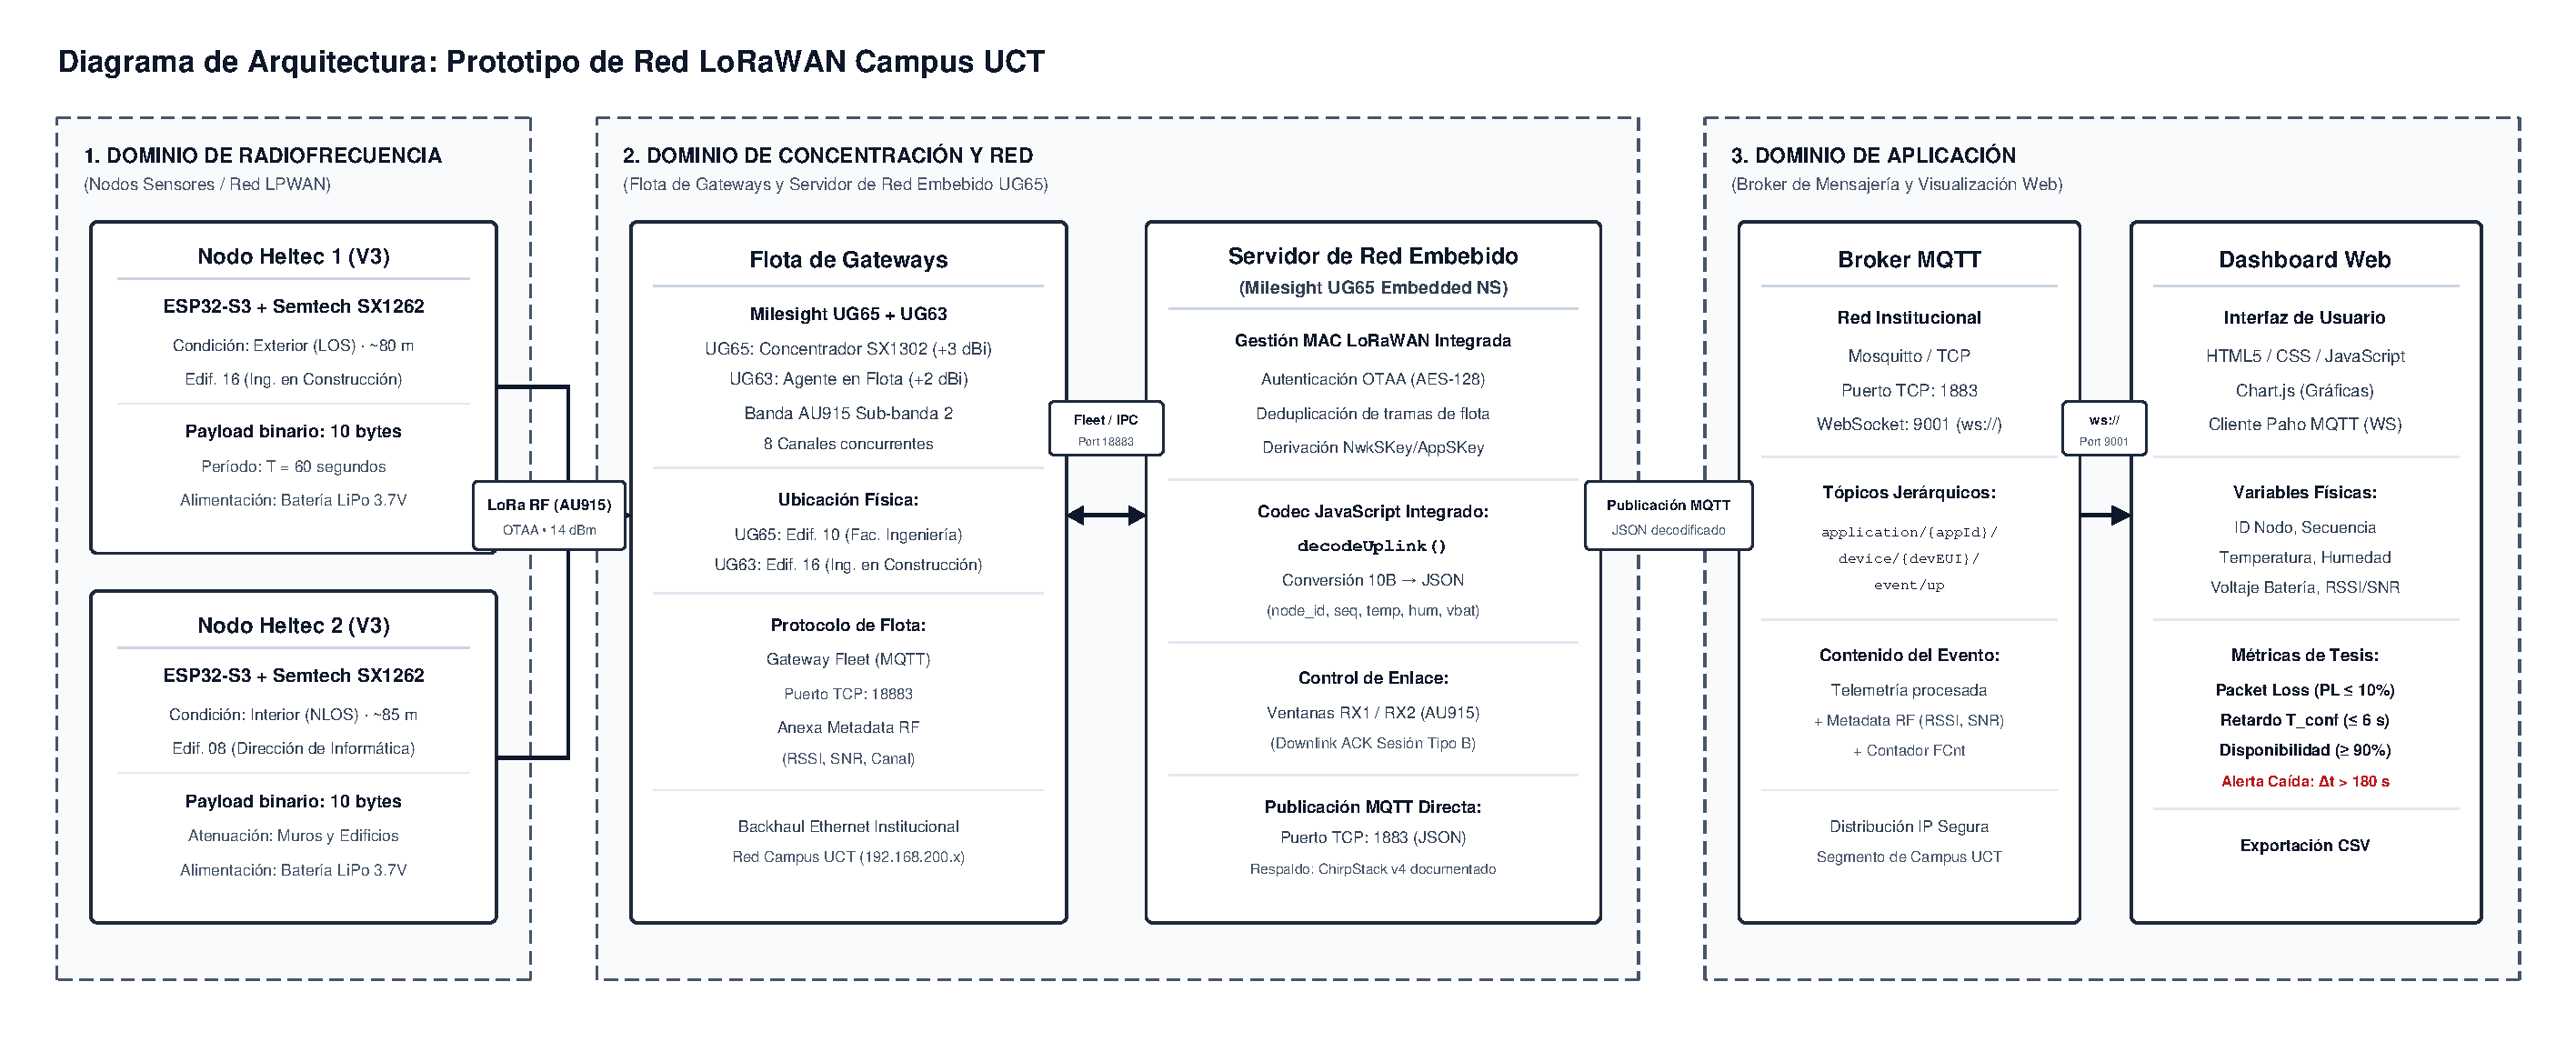
\includegraphics[width=\linewidth]{01_arquitectura_red}
\end{adjustwidth}
\caption{Diagrama de arquitectura general del prototipo de conectividad LoRaWAN intra-campus}
\label{fig:arquitectura-lorawan}
\end{figure}

Para garantizar rigor metodológico en la evaluación de calidad de servicio (RQS1 y RQS2), las
campañas experimentales se dividen en dos regímenes de capa MAC mutuamente excluyentes
(Figura~\ref{fig:secuencia-comunicacion}):

\begin{itemize}
  \item \textbf{Sesiones Tipo A -- Pérdida de paquetes ($PL$):} Emplean \emph{tramas no
  confirmadas} (\textit{unconfirmed data up}) con número de transmisiones fijado en $NbTrans = 1$.
  Esto impide reintentos automáticos en capa MAC y permite medir de manera directa la pérdida real
  inducida por la atenuación y el desvanecimiento del canal físico sobre lotes de 100 tramas.

  \item \textbf{Sesiones Tipo B -- Retardo de confirmación ($T_{\mathrm{conf}}$):} Emplean
  \emph{tramas confirmadas} (\textit{confirmed data up}), cronometrando en el propio
  microcontrolador el tiempo transcurrido desde el inicio del envío hasta la demodulación exitosa
  del acuse de recibo (\texttt{ACK}) transmitido por el servidor de red en las ventanas de
  recepción RX1 o RX2, sobre lotes mínimos de 30 tramas confirmadas.
\end{itemize}

\begin{figure}[H]
\centering
\begin{adjustwidth}{-1.2cm}{-1.2cm}
  \centering
  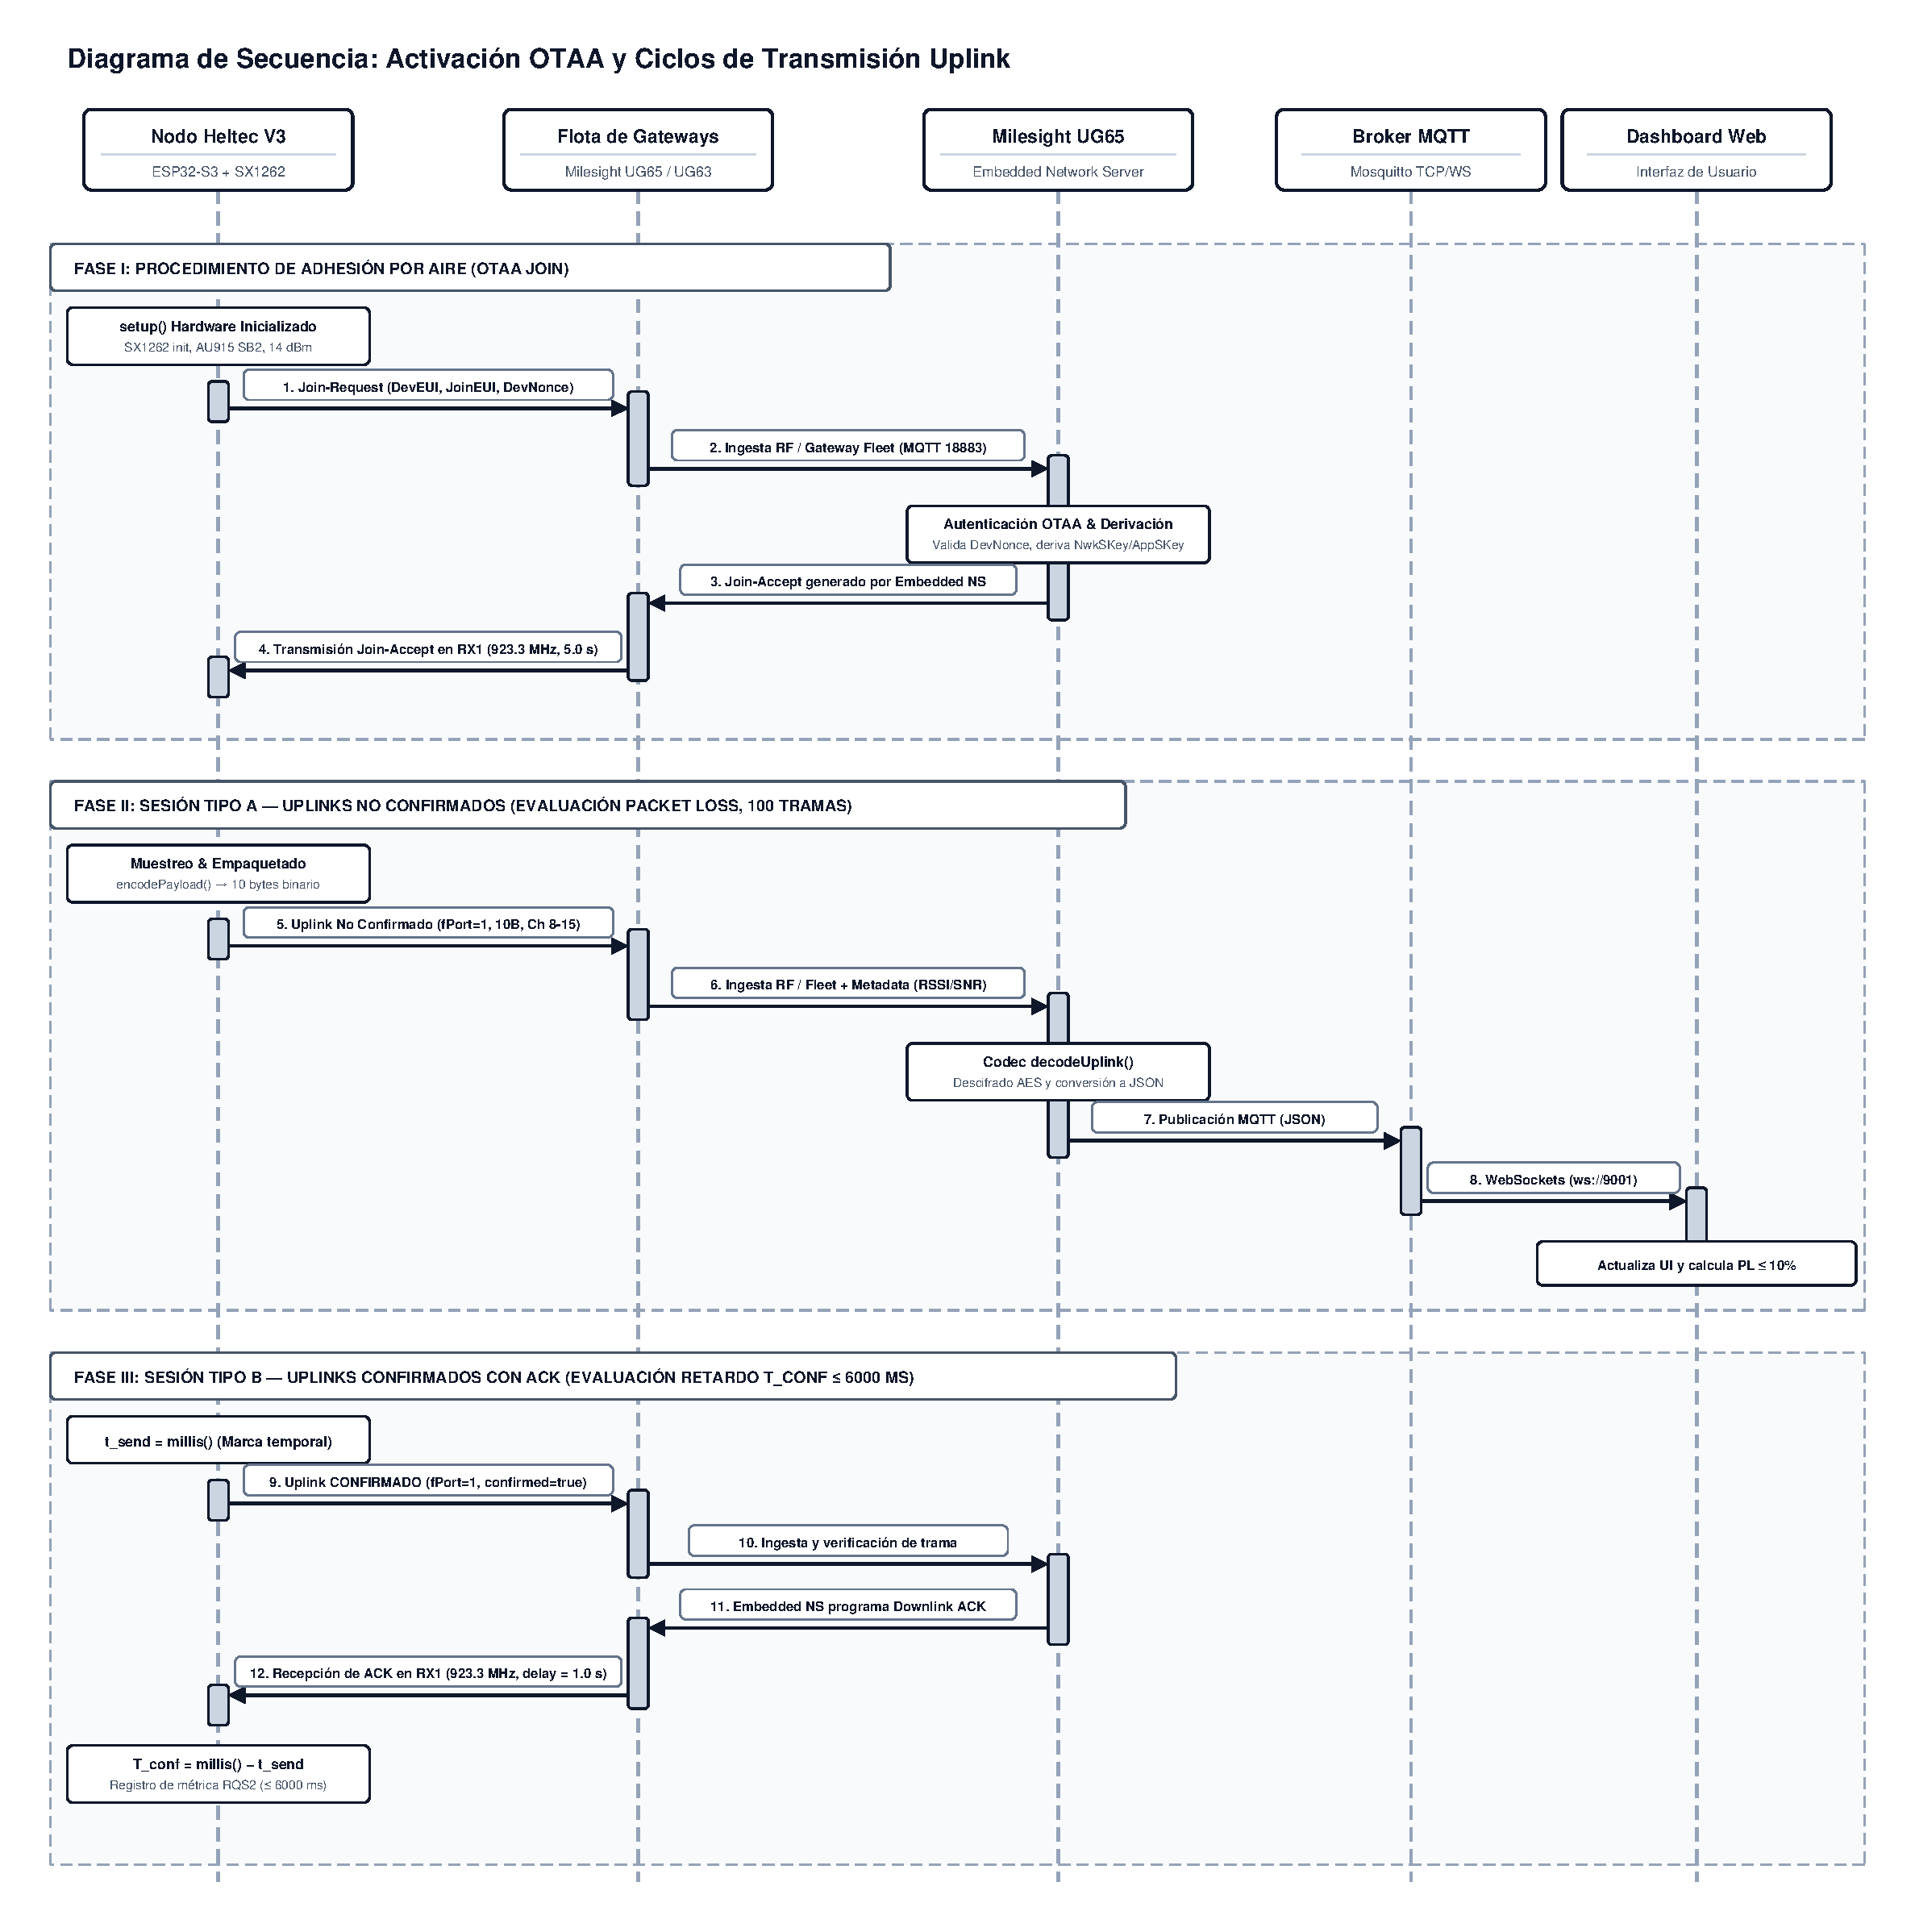
\includegraphics[width=\linewidth]{02_secuencia_otaa_uplink}
\end{adjustwidth}
\caption{Diagrama de secuencia de comunicaciones: activación OTAA, Sesiones Tipo A y Sesiones Tipo B}
\label{fig:secuencia-comunicacion}
\end{figure}

\section{Partes interesadas}

La gobernanza académica y operativa del proyecto distingue entre el patrocinador institucional y
los facilitadores técnicos (Cuadros~\ref{tab:stakeholders} y \ref{tab:validacion-stakeholders}). La
necesidad institucional es encabezada por la Dirección de la Carrera de Ingeniería Civil
Informática a través del Prof. Mario Villanueva, mientras que la provisión de equipamiento
LoRaWAN y espacio físico en laboratorio se articula directamente en el Departamento de Informática,
sumando además la sinergia directa con tesistas de proyectos IoT complementarios.

\begin{table}[H]
\centering
\caption{Partes interesadas y necesidades del proyecto}
\label{tab:stakeholders}
\small
\begin{tabularx}{\textwidth}{p{3.4cm} X X}
\toprule
\textbf{Stakeholder} & \textbf{Necesidad identificada} & \textbf{Implicancia en el proyecto}\\
\midrule
Dirección de Carrera / Profesor Guía (Prof. Mario Villanueva)
&
Validar empíricamente la viabilidad de una red LoRaWAN intra-campus y establecer una base tecnológica replicable en la Facultad de Ingeniería.
&
Aprueba el alcance, supervisa la implementación en laboratorio y valida los criterios SMART de aceptación.
\\
\midrule
Soporte Técnico / Laboratorio Departamento de Informática
&
Facilitar el equipamiento de concentración (Gateways Milesight), nodos Heltec y conectividad eléctrica/red local en el Edificio~10.
&
Permite la operación controlada del servidor embebido y la flota de gateways sin afectar servicios críticos del campus.
\\
\midrule
Proyectos de Título Complementarios (Vicente Ramírez)
&
Disponer de una capa física/MAC LoRaWAN estandarizada y un contrato de payload decodificado vía MQTT para alimentar plataformas superiores de gestión IoT.
&
Delimita claramente la frontera entre el transporte radioeléctrico (presente tesis) y la plataforma empresarial de monitoreo.
\\
\midrule
Estudiantes y futuros tesistas UCT
&
Contar con código fuente modular, códecs documentados y arquitecturas de respaldo (Embedded NS y ChirpStack v4) listas para reutilización.
&
Exige documentación rigurosa y versionamiento estructurado en GitHub.
\\
\bottomrule
\end{tabularx}
\end{table}

\begin{table}[H]
\centering
\caption{Consolidación de validación y soporte con partes interesadas}
\label{tab:validacion-stakeholders}
\small
\begin{tabularx}{\textwidth}{p{3.4cm} X X}
\toprule
\textbf{Actor} & \textbf{Coordinación ejecutada} & \textbf{Estado en Etapa 3}\\
\midrule
Dirección de Carrera (Prof. Mario Villanueva)
&
Validación del problema, acompañamiento presencial durante la puesta en marcha de gateways y nodos, y definición del escenario experimental en el campus.
&
Completado y validado en terreno (Agosto--Octubre 2026).
\\
\midrule
Laboratorio Depto. de Informática
&
Provisión efectiva de Gateways Milesight UG65 y UG63, placas Heltec WiFi LoRa 32 V3, sensores DHT11 y emplazamiento físico en Edificio~10.
&
Equipamiento operativo e integrado en red local de pruebas (Octubre 2026).
\\
\bottomrule
\end{tabularx}
\end{table}

% ============================================================
% CAPÍTULO 3: OBJETIVOS Y TRAZABILIDAD
% ============================================================
\chapter{Objetivos y Trazabilidad}

\section{Matriz de trazabilidad}

El Cuadro~\ref{tab:trazabilidad} vincula formalmente cada requerimiento funcional, técnico y de
calidad de servicio con los objetivos específicos, las partes interesadas y los mecanismos de
verificación empírica aplicados en la Etapa~3.

\begin{table}[H]
\centering
\caption{Matriz de trazabilidad entre problema, stakeholders, objetivos y requerimientos}
\label{tab:trazabilidad}
\tiny
\begin{tabularx}{\textwidth}{
  >{\bfseries\raggedright\arraybackslash}p{0.8cm}
  >{\raggedright\arraybackslash}p{1.5cm}
  >{\raggedright\arraybackslash}p{2.3cm}
  >{\raggedright\arraybackslash}X
  >{\raggedright\arraybackslash}X}
\toprule
\textbf{Req.} &
\textbf{Obj.} &
\textbf{Stakeholder} &
\textbf{Necesidad / problema} &
\textbf{Justificación y verificación}\\
\midrule
RF1 & O1, O4 &
Dirección de Carrera
&
Capturar variables reales y transmitir tramas desde los nodos sensores.
&
Base física del prototipo; verificado mediante lecturas DHT11 y tramas AU915 recibidas.
\\
\midrule
RF2 & O1, O2 &
Depto. de Informática
&
Concentrar, deduplicar y procesar las tramas LoRaWAN en el edificio central.
&
Verificado mediante la operación conjunta de la flota Milesight UG65 (Controlador) y UG63 (Agente).
\\
\midrule
RF3 & O2, O3 &
Depto. de Informática / Proyecto Complementario
&
Publicar tramas decodificadas hacia el entorno IP mediante protocolo estándar.
&
Verificado contrastando contadores de secuencia radio frente a publicaciones JSON en MQTT (puerto 1883).
\\
\midrule
RF4 & O3, O4 &
Dirección de Carrera / Tesista
&
Distinguir nodo de origen, estampa temporal, variables físicas y nivel RF en pantalla.
&
Verificado en el banco de pruebas local (Python/SQLite) con filtrado independiente por \texttt{DevEUI}.
\\
\midrule
RF5 & O4 &
Dirección de Carrera
&
Ejecutar campañas separadas Tipo~A y Tipo~B con registro reproducible.
&
Verificado mediante firmwares dedicados y exportación estructurada en base de datos \texttt{telemetry.db}.
\\
\midrule
RT1 & O1--O4 &
Marco Regulatorio (SUBTEL)
&
Operar dentro de banda y potencia legal exenta de concesión en Chile.
&
Configuración fija en AU915 SB2 (916,8--918,2~MHz) a $14\,\text{dBm}$ ($25\,\text{mW}$).
\\
\midrule
RT2--RT3 & O1--O4 &
Tesista / Laboratorio
&
Proteger transceptores RF y mantener estandarización de desarrollo en C++/Arduino IDE.
&
Verificación física de antenas previa a energización y 4 sketches modulares en repositorio GitHub.
\\
\midrule
RQS1 & O4 &
Tesista / Comisión Evaluadora
&
Cuantificar confiabilidad del enlace físico sin máscara de retransmisiones.
&
Cálculo empírico de $PL$ en Sesiones Tipo~A ($NbTrans=1$). Umbral: $PL \leq 10\%$.
\\
\midrule
RQS2 & O4 &
Tesista / Comisión Evaluadora
&
Cuantificar latencia bidireccional de confirmación en Clase~A.
&
Medición de $T_{\mathrm{conf}}$ en Sesiones Tipo~B (\textit{confirmed uplinks}). Umbral: $T_{\mathrm{conf}} \leq 6,0\,\text{s}$.
\\
\midrule
RQS3 & O4 &
Tesista / Comisión Evaluadora
&
Caracterizar continuidad temporal del servicio de telemetría.
&
Evaluación de intervalos entre recepciones ($\Delta t_{\mathrm{rec}} \leq 3\,T_{\mathrm{periodo}}$). Umbral: $A \geq 90\%$.
\\
\bottomrule
\end{tabularx}
\end{table}

% ============================================================
% CAPÍTULO 4: ESPECIFICACIÓN DE REQUERIMIENTOS Y MODELO EXPERIMENTAL
% ============================================================
\chapter{Especificación de Requerimientos}

\section{Requerimientos funcionales}

\begin{table}[H]
\centering
\caption{Requerimientos funcionales del prototipo}
\label{tab:rf}
\scriptsize
\begin{tabularx}{\textwidth}{
  >{\bfseries\raggedright\arraybackslash}p{0.8cm}
  >{\raggedright\arraybackslash}X
  >{\raggedright\arraybackslash}p{2.5cm}
  >{\raggedright\arraybackslash}p{1.4cm}
  >{\raggedright\arraybackslash}p{2.4cm}
}
\toprule
\textbf{ID} &
\textbf{Requerimiento} &
\textbf{Justificación} &
\textbf{Obj.} &
\textbf{Verificación}\\
\midrule
RF1 &
Los nodos sensores (al menos dos) deben capturar datos ambientales reales y transmitir tramas
binarias mediante el protocolo LoRaWAN AU915 Sub-banda~2.
&
Función elemental que habilita la evaluación empírica del canal.
&
O1, O4
&
Prueba de transmisión y registro en SQLite.
\\
\midrule
RF2 &
La infraestructura Gateway LoRaWAN debe demodular, autenticar (OTAA) y procesar las tramas
provenientes de los nodos sensores desplegados en el campus.
&
Punto central de concentración de la topología en estrella.
&
O1, O2
&
Registros del servidor embebido UG65.
\\
\midrule
RF3 &
El sistema debe decodificar el payload binario y publicar hacia la red IP las tramas válidas
mediante un broker MQTT.
&
Desacopla la red de radiofrecuencia de las capas de persistencia y visualización.
&
O2, O3
&
Suscripción MQTT y persistencia automática.
\\
\midrule
RF4 &
El dashboard local de laboratorio debe identificar cada nodo sensor y mostrar identificador,
marca temporal, temperatura, humedad, batería, RSSI y SNR.
&
Permite supervisar en tiempo real las pruebas de campo y auditar la salud del enlace.
&
O3, O4
&
Interfaz web operativa y base de datos local.
\\
\midrule
RF5 &
El sistema debe permitir ejecutar sesiones de tráfico controlado Tipo~A (no confirmadas) y
Tipo~B (confirmadas) con configuraciones independientes y exportables.
&
Asegura reproducibilidad científica sin interferencia entre métricas MAC.
&
O4
&
Sketches separados y exportación CSV por sesión.
\\
\bottomrule
\end{tabularx}
\end{table}

\section{Requerimientos no funcionales y restricciones}

\begin{table}[H]
\centering
\caption{Requerimientos no funcionales, restricciones y criterios de verificación}
\label{tab:rnf}
\scriptsize
\setlength{\tabcolsep}{3.5pt}
\renewcommand{\arraystretch}{1.05}
\begin{tabularx}{\textwidth}{
  >{\bfseries\raggedright\arraybackslash}p{0.85cm}
  >{\raggedright\arraybackslash}p{1.6cm}
  >{\raggedright\arraybackslash}X
  >{\raggedright\arraybackslash}p{2.5cm}
  >{\raggedright\arraybackslash}p{2.1cm}
}
\toprule
\textbf{ID} &
\textbf{Categoría} &
\textbf{Requisito} &
\textbf{Justificación} &
\textbf{Verificación}\\
\midrule
RT1 &
Tecnología / normativa &
Operación exclusiva bajo el plan regional AU915 (915--928~MHz) con potencia máxima de $14\,\text{dBm}$ ($25\,\text{mW}$), conforme a la normativa SUBTEL \parencite{subtel2017,subtel737_2025}.
&
Asegura legalidad radioeléctrica en territorio chileno sin requerir concesión.
&
Inspección de firmware y configuración RF del gateway.
\\
\midrule
RT2 &
Hardware &
Conexión obligatoria de antenas de $915\,\text{MHz}$ en nodos Heltec y gateways previo a toda energización.
&
Previene daño térmico por potencia reflejada en los transceptores SX1262/SX1302.
&
Protocolo de verificación física en laboratorio.
\\
\midrule
RT3 &
Desarrollo &
Desarrollo íntegro del firmware de los nodos sensores en lenguaje C/C++ utilizando Arduino IDE y librería RadioLib.
&
Estandariza la mantenibilidad del código para futuros estudiantes del departamento.
&
Inspección del repositorio GitHub oficial.
\\
\midrule
RQS1 &
Calidad de servicio &
Tasa de pérdida de paquetes calculada en Sesiones Tipo~A ($NbTrans = 1$) con umbral de viabilidad $PL \leq 10\%$ \parencite{kaur2024campus,ahmed2024vegetacion}.
&
Cuantifica la confiabilidad pura del enlace radioeléctrico intra-campus.
&
Conteo de secuencias enviadas versus recibidas.
\\
\midrule
RQS2 &
Calidad de servicio &
Retardo de confirmación medido en Sesiones Tipo~B (\textit{confirmed uplinks}) con umbral $T_{\mathrm{conf}} \leq 6,0\,\text{s}$ \parencite{lorawan1_0_4}.
&
Verifica la viabilidad del canal descendente (\textit{downlink}) en ventanas RX1/RX2.
&
Cronometraje diferencial $T_{\mathrm{ACK}} - T_{\mathrm{env}}$.
\\
\midrule
RQS3 &
Calidad de servicio &
Disponibilidad temporal del enlace estacionario con umbral $A \geq 90\%$, declarando caída cuando $\Delta t_{\mathrm{rec}} > 3 \cdot T_{\mathrm{periodo}}$ \parencite{barrachina2023campus}.
&
Evalúa la ausencia de desconexiones prolongadas durante las campañas.
&
Serie temporal de marcas de recepción en SQLite.
\\
\bottomrule
\end{tabularx}
\end{table}

\section{Formulación matemática de las métricas de evaluación}

\subsection{Pérdida de paquetes (\textit{Packet Loss})}

\begin{equation}
PL(\%) =
100\left(
1-\frac{N_{\mathrm{rec}}}{N_{\mathrm{env}}}
\right)
\label{eq:packetloss}
\end{equation}

donde $N_{\mathrm{env}}$ corresponde al total de tramas físicas emitidas por el nodo (determinado
mediante el diferencial del contador de secuencia incremental de aplicación/MAC con $NbTrans = 1$)
y $N_{\mathrm{rec}}$ corresponde al número de tramas únicas demoduladas con éxito.

\subsection{Tiempo de confirmación del uplink ($T_{\mathrm{conf}}$)}

\begin{equation}
T_{\mathrm{conf}} = T_{\mathrm{ACK}} - T_{\mathrm{env}}
\label{eq:tconf}
\end{equation}

donde $T_{\mathrm{env}}$ marca el inicio de la transmisión confirmada en el nodo Heltec~V3 y
$T_{\mathrm{ACK}}$ el instante exacto en que el transceptor SX1262 valida el paquete descendente
con el bit \texttt{ACK} activo en la ventana RX1 ($\approx 1\,\text{s}$) o RX2 ($\approx 2\,\text{s}$).

\subsection{Disponibilidad del enlace ($A$)}

\begin{equation}
A(\%) =
100\left(1 - \frac{\sum T_{\text{ca\'{\i}da}}}{T_{\text{prueba}}}\right),
\qquad \text{con estado de ca\'{\i}da si } \Delta t_{\text{rec}} > 3 \cdot T_{\text{periodo}}
\label{eq:availability}
\end{equation}

donde $T_{\text{prueba}}$ es la duración total de la ventana experimental y $T_{\text{periodo}}$ es
el intervalo nominal de envío configurado en la sesión.

\section{Protocolo experimental y estructura de payload}
\label{sec:protocolo-experimental}

El Cuadro~\ref{tab:protocolo} sintetiza los parámetros del protocolo experimental consolidado para
las campañas de evaluación, mientras que la Figura~\ref{fig:flujo-payload} detalla la estructura
binaria de 10~bytes y su pipeline de decodificación extremo a extremo.

\begin{table}[H]
\centering
\caption{Parámetros del protocolo experimental consolidado para las sesiones de evaluación}
\label{tab:protocolo}
\small
\setlength{\tabcolsep}{4pt}
\renewcommand{\arraystretch}{1.2}
\begin{tabularx}{\textwidth}{
  >{\raggedright\arraybackslash}p{4.8cm}
  >{\raggedright\arraybackslash}X
}
\toprule
\textbf{Parámetro} & \textbf{Valor consolidado / condición operativa}\\
\midrule
\textbf{Ubicación Concentración} &
Edificio~10 (Facultad de Ingeniería -- Departamento de Informática), instalación interior en planta docente.\\
\midrule
\textbf{Nodo 1 (condición LOS)} &
Edificio~16, con línea de vista directa hacia el Edificio~10. Distancia aproximada de referencia: $\approx 80\,\text{m}$.\\
\midrule
\textbf{Nodo 2 (condición NLOS)} &
Edificio~08, con obstrucción estructural interpuesta por el Edificio~09. Distancia aproximada homologada: $\approx 85\,\text{m}$.\\
\midrule
\textbf{Potencia de transmisión} &
$14\,\text{dBm}$ ($25\,\text{mW}$, norma SUBTEL Res. Exenta N.º 1.985/2017 \parencite{subtel2017}).\\
\midrule
\textbf{Plan y Parámetros RF} &
AU915 Sub-banda~2 (canales 8--15: $916,8\text{--}918,2\,\text{MHz}$), $\text{BW} = 125\,\text{kHz}$, SF7 (DR5) inicial.\\
\midrule
\textbf{Payload binario} &
10~bytes en formato \textit{Big-Endian}: \texttt{NodeID} (1~B), \texttt{Seq} (4~B), \texttt{Temp$\times$100} (2~B), \texttt{Hum$\times$100} (2~B), \texttt{Bat} (1~B).\\
\midrule
\textbf{Cadencia de envío} &
$15\,\text{s}$ en pruebas preliminares aceleradas Tipo~A ($12\,\text{s}$ post-ACK en Tipo~B); configurable a $60\,\text{s}$ en operación nominal.\\
\midrule
\textbf{Sesiones Tipo A ($PL$)} &
100 tramas no confirmadas por sesión ($NbTrans = 1$); 3 repeticiones por condición (mañana, mediodía y tarde en Etapa~4).\\
\midrule
\textbf{Sesiones Tipo B ($T_{\mathrm{conf}}$)} &
$\geq 30$ tramas confirmadas (\textit{confirmed uplinks}) por sesión con medición de ventana RX1/RX2.\\
\bottomrule
\end{tabularx}
\end{table}

\begin{figure}[H]
\centering
\begin{adjustwidth}{-1.4cm}{-1.4cm}
  \centering
  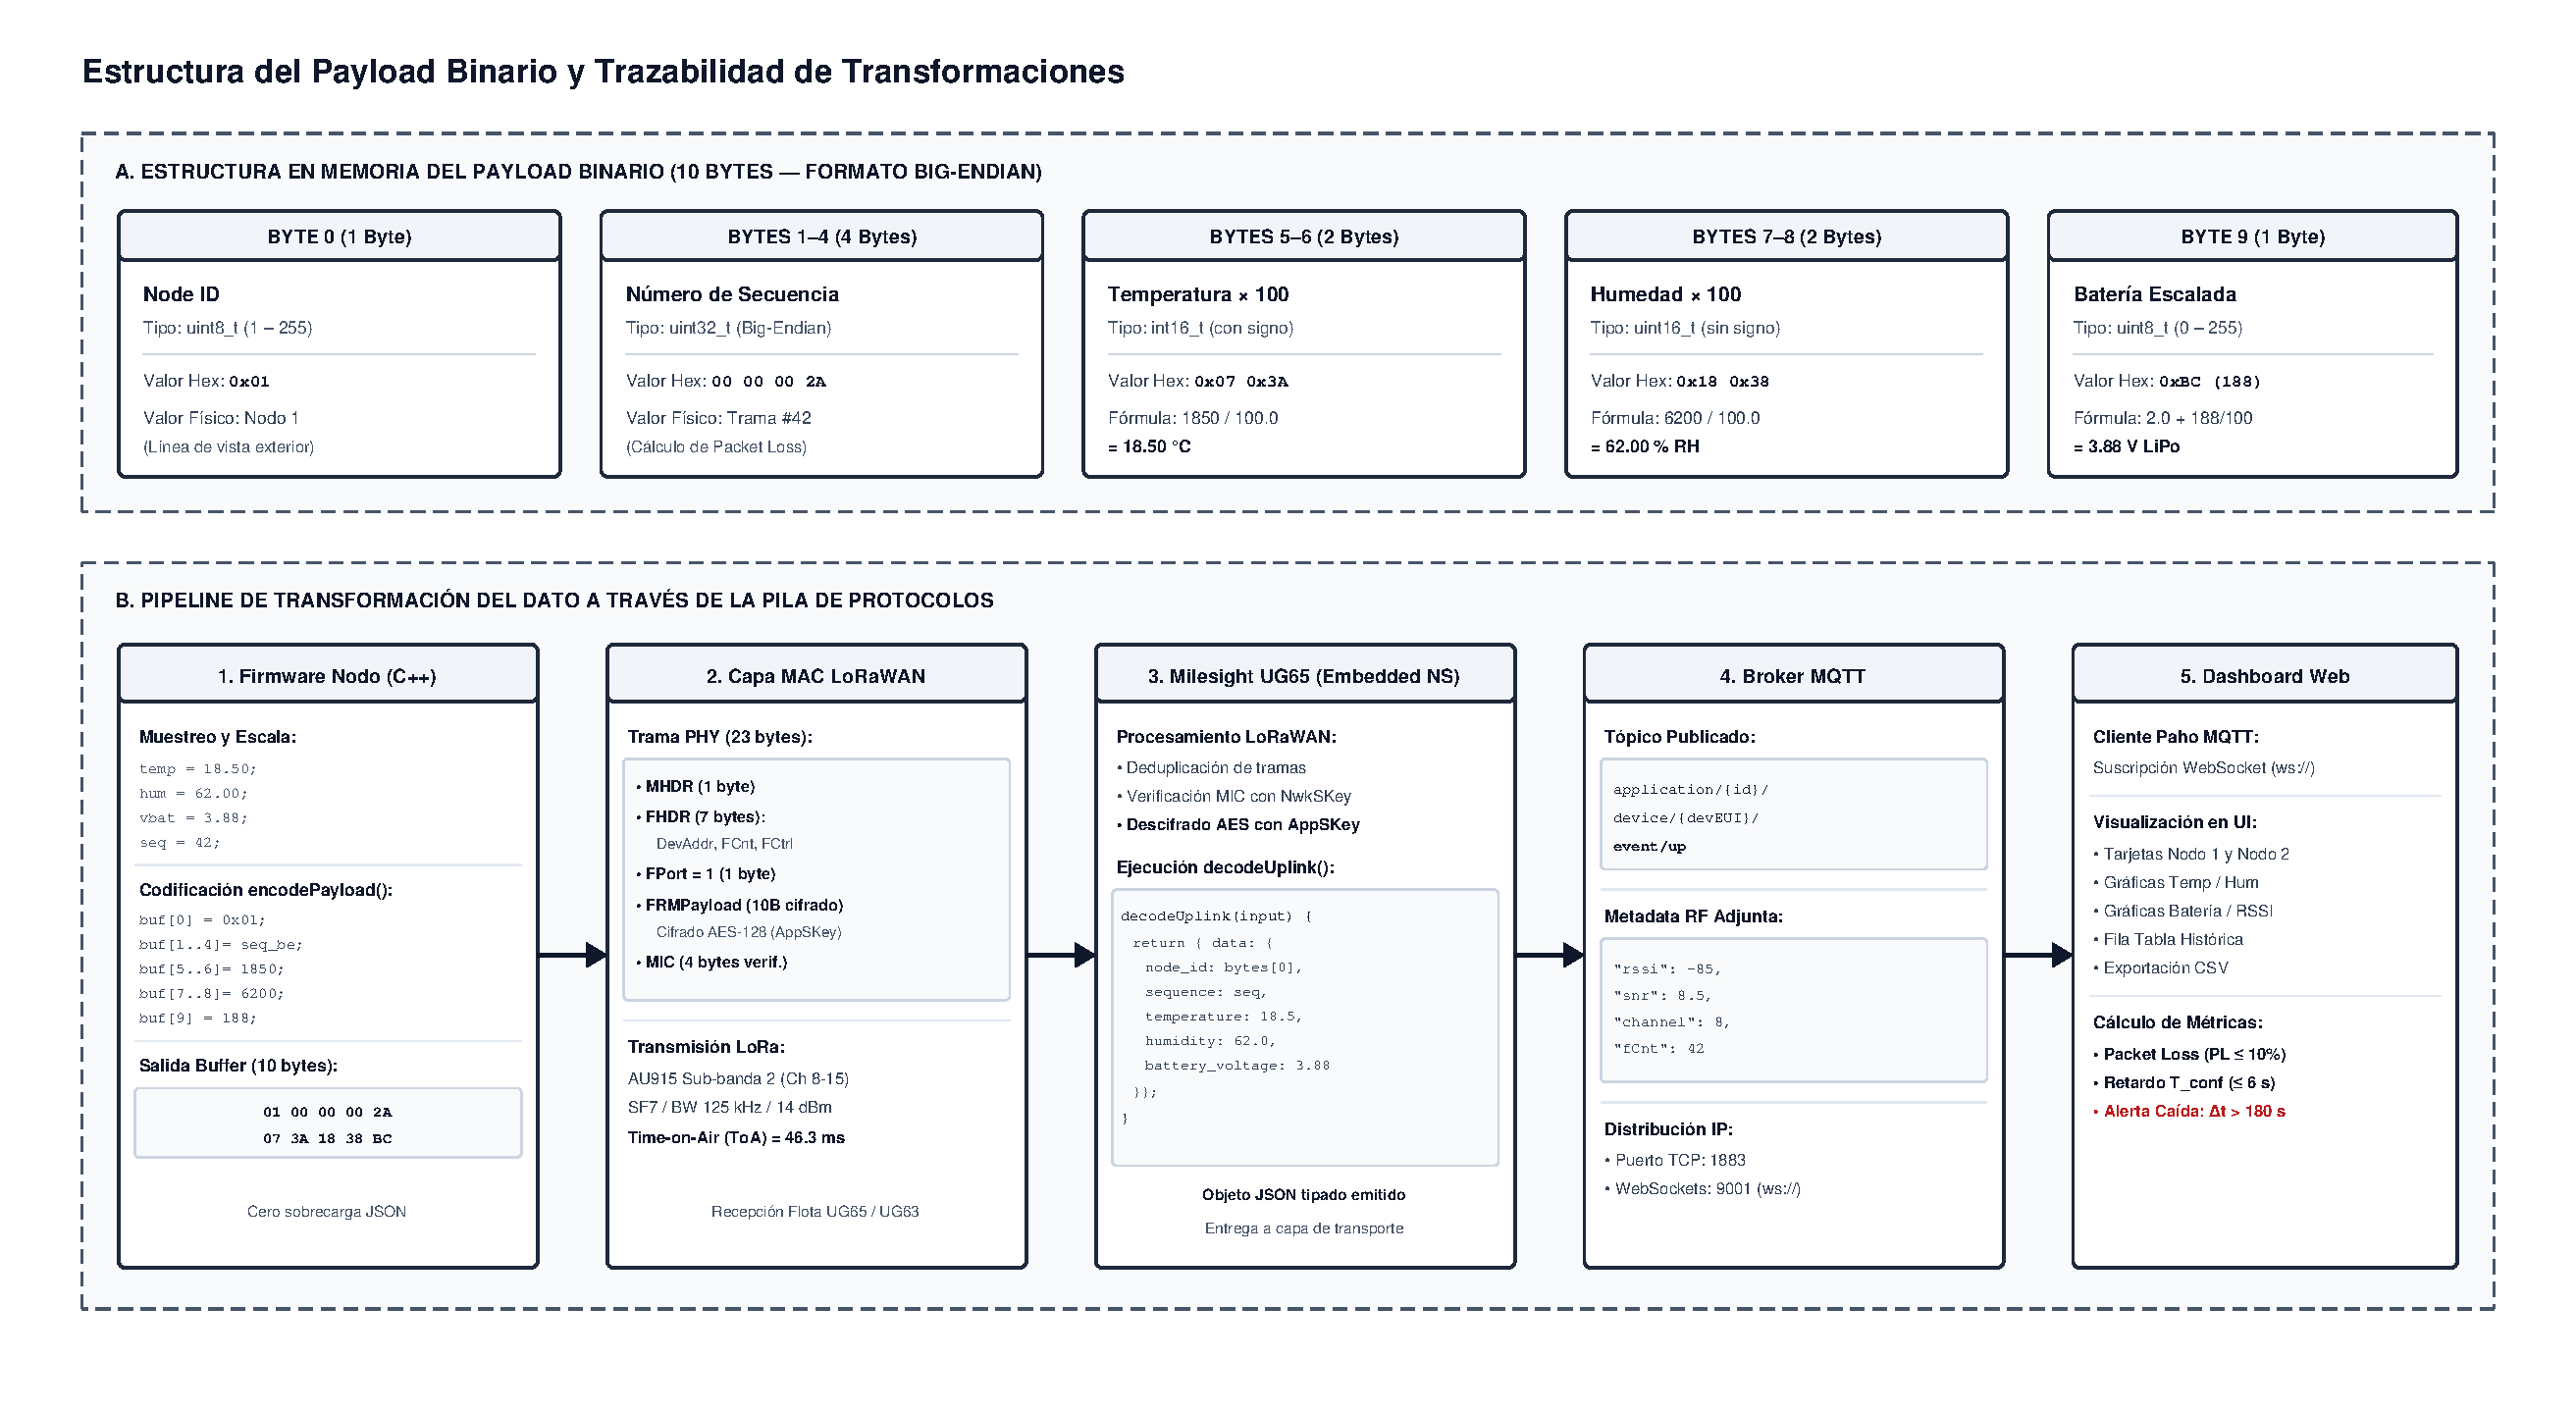
\includegraphics[width=\linewidth]{03_flujo_payload}
\end{adjustwidth}
\caption{Estructura del payload binario de 10~bytes y pipeline de procesamiento extremo a extremo}
\label{fig:flujo-payload}
\end{figure}

\section{Fundamento teórico de propagación y evaluación de alternativas}

El análisis de radioenlace parte del balance de potencia general:
\begin{equation}
P_r = P_t + G_t + G_r - L_p - L_s
\label{eq:linkbudget}
\end{equation}
donde $P_t = 14\,\text{dBm}$ es la potencia de transmisión, $G_t \approx 2\,\text{dBi}$ y
$G_r \approx 2\,\text{dBi}$ son las ganancias de las antenas omnidireccionales, $L_p$ es la pérdida
de trayectoria y $L_s$ agrupa las pérdidas de inserción. Si bien la pérdida en espacio libre
(\textit{Free Space Path Loss}, FSPL) \parencite{seybold2005}:
\begin{equation}
L_{\mathrm{FSPL}} = 20\log_{10}(d_{\mathrm{km}}) + 20\log_{10}(f_{\mathrm{MHz}}) + 32,44
\label{eq:fspl}
\end{equation}
entrega una cota inferior teórica (aproximadamente $69,7\,\text{dB}$ a $d = 0,08\,\text{km}$ y
$f = 916,8\,\text{MHz}$), la presencia de edificios interpuestos en el campus exige emplear el
\textbf{modelo log-distancia con desvanecimiento lento por sombra (\textit{shadowing})}
\parencite{rademacher2021,ahmed2024vegetacion}:
\begin{equation}
PL(d) = PL(d_0) + 10\,n\,\log_{10}\left(\frac{d}{d_0}\right) + X_\sigma
\label{eq:logdistance}
\end{equation}
donde $d_0 = 1\,\text{m}$ es la distancia de referencia, $n$ es el exponente de pérdida de
trayectoria ($n \approx 2,0$ en LOS despejado y $n \in [2,7;\,4,5]$ en recintos universitarios
construidos) y $X_\sigma \sim \mathcal{N}(0, \sigma^2)$ modela en decibelios la atenuación por
obstáculos estructurales. Finalmente, el Cuadro~\ref{tab:alternativas} resume la comparación
crítica frente a otras alternativas tecnológicas evaluadas en la fase de preparación.

\begin{table}[H]
\centering
\caption{Comparación crítica de alternativas de conectividad para el caso de estudio}
\label{tab:alternativas}
\tiny
\begin{tabularx}{\textwidth}{
  >{\raggedright\arraybackslash}p{2.5cm}
  >{\raggedright\arraybackslash}X
  >{\raggedright\arraybackslash}X
  >{\raggedright\arraybackslash}X
  >{\raggedright\arraybackslash}X}
\toprule
\textbf{Criterio} &
\textbf{Wi-Fi (IEEE 802.11)} &
\textbf{Celular (LTE-M/NB-IoT)} &
\textbf{Satelital IoT} &
\textbf{LoRaWAN (AU915)}\\
\midrule
Dependencia de terceros &
Depende de la red de AP institucionales y gestión TI central. &
Depende de cobertura y contrato con operador móvil comercial. &
Depende íntegramente de proveedor satelital externo. &
Opera sobre infraestructura propia administrada por el departamento. \\
\midrule
Consumo energético &
Elevado en asociación y TX (centenares de mA) \parencite{callebaut2020}. &
Moderado, superior a LPWAN no licenciadas durante sincronización. &
Elevado requerimiento de potencia radiada hacia órbita. &
Muy bajo consumo (decenas de mA por $<50\,\text{ms}$ en SF7). \\
\midrule
Penetración intra-campus &
Limitada en exteriores alejados y muros gruesos en $2,4/5\,\text{GHz}$. &
Buena penetración, pero con costos recurrentes por nodo. &
Nula operatividad en interiores (\textit{indoor}) sin vista al cielo. &
Alta sensibilidad (hasta $-137\,\text{dBm}$) y operación sub-ruido en banda sub-GHz. \\
\midrule
Costo operativo &
Sin cobro por trama, pero costoso de extender a patios/cubiertas. &
Suscripción recurrente por tarjeta SIM/dispositivo. &
Tarifa recurrente por mensaje transmitido. &
Costo operativo marginal nulo en banda libre ISM ($915\text{--}928\,\text{MHz}$). \\
\bottomrule
\end{tabularx}
\end{table}

% ============================================================
% CAPÍTULO 5: DISEÑO DE LA SOLUCIÓN
% ============================================================
\chapter{Diseño de la Solución}\label{cap:diseno-solucion}

\section{Introducción al diseño y consideraciones metodológicas}

El presente capítulo documenta la línea base de la fase de \textit{Diseño} (Fase~3 de la
metodología PPDIOO), transformando los requerimientos funcionales, no funcionales y criterios SMART
en una especificación de ingeniería modular y reproducible. Se formalizan aquí los parámetros
radioeléctricos bajo normativa chilena, el plan de frecuencias LoRaWAN AU915 Sub-banda~2, el
modelo criptográfico OTAA, la estructura del payload binario de 10~bytes y la arquitectura lógica de
integración de software sobre la cual se ejecutaron posteriormente las optimizaciones físicas de la
Etapa~3 (detalladas en el Capítulo~\ref{cap:implementacion-etapa3}).

\section{Diseño inicial de infraestructura y escenarios de propagación}\label{sec:despliegue-hardware}

\subsection{Emplazamiento central y especificación base de concentración}

El punto central de concentración radioeléctrica se proyectó en dependencias interiores del
\textbf{Departamento de Informática} (Edificio~10, Facultad de Ingeniería, Campus Dr. Luis Rivas del
Canto), recinto que provee alimentación eléctrica continua, resguardo físico y conectividad directa
hacia la red local de laboratorio. En la formulación original de la Etapa~2 se dimensionó como
unidad base un concentrador compacto \textit{indoor} Milesight UG63 (\texttt{UG63-L08GL-915M})
\parencite{milesight_ug63}, equipado con el procesador en banda base Semtech SX1302 de 8 canales
simultáneos \parencite{semtech_sx1302}, antena interna omnidireccional de $+2\,\text{dBi}$,
identificador único \texttt{C0BA1FFFFE0377FA} y soporte de transporte IP tanto por UDP Packet
Forwarder (puerto 1700 hacia ChirpStack v4) como por enlace MQTT de flota Milesight.

\subsection{Modelamiento analítico de escenarios LOS y NLOS}

Para aislar el efecto de la obstrucción estructural sobre el enlace radioeléctrico, el diseño
estableció dos condiciones contrastantes:
\begin{enumerate}
    \item \textbf{Condición LOS (\textit{Line-of-Sight} -- Línea de Vista Directa):} Trayectoria
    exterior despejada entre el edificio de concentración y el punto de medición, asegurando el
    despeje de al menos el $60\%$ de la primera Zona de Fresnel. Para una distancia representativa
    $d = 80\,\text{m}$ operando en $f = 916,8\,\text{MHz}$, el radio máximo en el punto medio del
    elipsoide de Fresnel viene dado por la Ecuación~\eqref{eq:fresnel-calc}:
    \begin{equation}\label{eq:fresnel-calc}
        r_1 = \frac{1}{2} \sqrt{\frac{c \cdot d}{f}}
        \approx \frac{1}{2} \sqrt{\frac{3 \times 10^8\,\text{m/s} \cdot 80\,\text{m}}{916,8 \times 10^6\,\text{Hz}}}
        \approx 2,56\,\text{m}
    \end{equation}
    Esta condición actúa como grupo de control experimental ($n \approx 2,0$).

    \item \textbf{Condición NLOS (\textit{Non-Line-of-Sight} -- Sin Línea de Vista):} Trayectoria a
    distancia geométrica equivalente, pero bloqueada por al menos un edificio completo de hormigón
    armado, tabiquería metálica y ventanales termopanel interpuestos en el eje directo hacia el
    concentrador, induciendo mecanismos combinados de atenuación por penetración, difracción en
    aristas y desvanecimiento por sombra (\textit{shadowing}).
\end{enumerate}

\section{Marco regulatorio y planificación radioeléctrica}\label{sec:marco-regulatorio}

\subsection{Normativa nacional SUBTEL (Chile)}

La operación radioeléctrica del prototipo se enmarca rigurosamente en la regulación vigente de la
Subsecretaría de Telecomunicaciones de Chile (SUBTEL):
\begin{itemize}
    \item \textbf{Resolución Exenta N.º 1.985 de 2017 de la SUBTEL} \parencite{subtel2017}: Fija la
    norma técnica de equipos de alcance reducido. En su Artículo~1, literal~j), habilita el uso sin
    concesión de la banda ISM de \textbf{$915\,\text{MHz}$ a $928\,\text{MHz}$} con límites de
    potencia radiada aparente de hasta $500\,\text{mW}$ p.i.r.e. ($+27\,\text{dBm}$), o hasta
    $1\,\text{W}$ ($+30\,\text{dBm}$) empleando técnicas de modulación digital de espectro
    ensanchado.
    \item \textbf{Resolución Exenta N.º 737 de 2025 de la SUBTEL} \parencite{subtel737_2025}:
    Actualiza los mecanismos de trazabilidad y certificación de equipos de alcance reducido en el
    país.
\end{itemize}

Tanto los gateways como los nodos Heltec WiFi LoRa 32 V3 se fijan por software en una potencia de
salida conducida de \textbf{$14\,\text{dBm}$ ($25\,\text{mW}$)} con antenas de $+2\,\text{dBi}$
($\text{p.i.r.e.} \approx 16\,\text{dBm}$), manteniendo un margen de resguardo superior a
$11\,\text{dB}$ por debajo del techo normativo chileno.

\subsection{Parametrización regional LoRaWAN: Plan AU915 Sub-banda 2}

Conforme a la especificación RP002-1.0.4 de la LoRa Alliance \parencite{lorawan_rp002}, el sistema
restringe su máscara de canales (\textit{Channel Mask}) exclusivamente a la \textbf{Sub-banda~2
(SB2)} del plan AU915, evitando barridos infructuosos en los 56 canales restantes durante el
procedimiento de asociación. El detalle frecuencial se presenta en el
Cuadro~\ref{tab:frecuencias-au915-diseno}.

\begin{table}[H]
\centering
\small
\caption{Plan de frecuencias y canales configurados en AU915 Sub-banda 2 (SB2)}\label{tab:frecuencias-au915-diseno}
\begin{tabularx}{\textwidth}{>{\raggedright\arraybackslash}p{2.4cm} >{\centering\arraybackslash}p{2.3cm} >{\centering\arraybackslash}p{2.0cm} >{\centering\arraybackslash}p{2.5cm} >{\raggedright\arraybackslash}X}
\toprule
\textbf{Canal / Enlace} & \textbf{Frecuencia} & \textbf{Ancho Banda} & \textbf{Data Rate} & \textbf{Función Operativa} \\
\midrule
Canal 08 (Up) & $916,80\,\text{MHz}$ & $125\,\text{kHz}$ & DR0--DR5 & Telemetría LoRaWAN (Tipo~A / B) \\
Canal 09 (Up) & $917,00\,\text{MHz}$ & $125\,\text{kHz}$ & DR0--DR5 & Telemetría LoRaWAN (Tipo~A / B) \\
Canal 10 (Up) & $917,20\,\text{MHz}$ & $125\,\text{kHz}$ & DR0--DR5 & Telemetría LoRaWAN (Tipo~A / B) \\
Canal 11 (Up) & $917,40\,\text{MHz}$ & $125\,\text{kHz}$ & DR0--DR5 & Telemetría LoRaWAN (Tipo~A / B) \\
Canal 12 (Up) & $917,60\,\text{MHz}$ & $125\,\text{kHz}$ & DR0--DR5 & Telemetría LoRaWAN (Tipo~A / B) \\
Canal 13 (Up) & $917,80\,\text{MHz}$ & $125\,\text{kHz}$ & DR0--DR5 & Telemetría LoRaWAN (Tipo~A / B) \\
Canal 14 (Up) & $918,00\,\text{MHz}$ & $125\,\text{kHz}$ & DR0--DR5 & Telemetría LoRaWAN (Tipo~A / B) \\
Canal 15 (Up) & $918,20\,\text{MHz}$ & $125\,\text{kHz}$ & DR0--DR5 & Telemetría LoRaWAN (Tipo~A / B) \\
\midrule
Canal 65 (Up) & $917,50\,\text{MHz}$ & $500\,\text{kHz}$ & DR6 (SF8) & Canal rápido de banda ancha \\
\midrule
Bajada RX1    & $923,30\text{--}927,50\,\text{MHz}$ & $500\,\text{kHz}$ & DR8--DR13 & Recepción Join-Accept y ACK ($1\,\text{s}$) \\
Bajada RX2    & $923,30\,\text{MHz}$ & $500\,\text{kHz}$ & DR8 (SF12) & Ventana secundaria de respaldo ($2\,\text{s}$) \\
\bottomrule
\end{tabularx}
\vspace{0.15cm}
\footnotesize
\textit{Nota:} En AU915, DR5 corresponde a SF7/$125\,\text{kHz}$ y DR0 a SF12/$125\,\text{kHz}$. La ventana RX1 se mapea módulo 8 sobre los canales descendentes de $500\,\text{kHz}$ ($923,30\,\text{MHz}$ para el Canal~08), mientras que RX2 permanece fija en $923,30\,\text{MHz}$ con SF12.
\end{table}

\subsection{Seguridad criptográfica y activación OTAA}

La autenticación de dispositivos emplea exclusivamente \textit{Over-The-Air Activation} (OTAA) bajo
LoRaWAN 1.0.4 \parencite{lorawan1_0_4}. Cada nodo físico almacena un \texttt{DevEUI} único de
64~bits, un \texttt{JoinEUI} (\texttt{0000000000000000}) y una clave raíz simétrica AES-128
(\texttt{AppKey}). En cada asociación (\textit{Join-Request} / \textit{Join-Accept}) se verifica el
código de integridad de mensaje (\texttt{MIC}, AES-CMAC de 4~bytes) y se derivan llaves efímeras
independientes para integridad MAC (\texttt{NwkSKey}) y cifrado extremo a extremo del payload
(\texttt{AppSKey}), reiniciando los contadores \texttt{FCntUp} y \texttt{FCntDown} contra ataques de
repetición (\textit{replay attacks}).

\section{Especificación del payload binario e interfaces de datos}\label{sec:interfaces-software}

Para minimizar el tiempo de ocupación del canal (\textit{Time-on-Air}) y evitar la sobrecarga de
transmitir cadenas ASCII o JSON por radiofrecuencia, se especifica un formato binario determinista
de 10~bytes en ordenamiento \textit{Big-Endian} sobre \texttt{FPort = 1}:
\begin{equation}
\text{Payload}_{10\text{B}} =
\underbrace{[B_0]}_{\text{NodeID}} \;
\underbrace{[B_1, B_2, B_3, B_4]}_{\text{Seq (uint32 BE)}} \;
\underbrace{[B_5, B_6]}_{T_{\text{raw}} = \lfloor T \cdot 100 \rfloor} \;
\underbrace{[B_7, B_8]}_{H_{\text{raw}} = \lfloor H \cdot 100 \rfloor} \;
\underbrace{[B_9]}_{V_{\text{raw}} = \lfloor (V_{\text{bat}} - 2,0) \cdot 100 \rfloor}
\label{eq:payload-10b}
\end{equation}

Una vez demodulada la trama y decodificado el vector binario en el servidor de red, el mensaje se
publica vía MQTT \parencite{oasis_mqtt} hacia el puerto TCP~1883 entregando tanto las variables de
aplicación como los metadatos físicos de radioenlace (RSSI, SNR, \texttt{fCnt} y \texttt{devEUI}).
El Cuadro~\ref{tab:dashboard-kpis-diseno} sintetiza las variables supervisadas en el entorno de
monitoreo.

\begin{table}[H]
\centering
\small
\caption{Matriz de variables físicas y métricas radioeléctricas supervisadas}\label{tab:dashboard-kpis-diseno}
\begin{tabularx}{\textwidth}{>{\raggedright\arraybackslash}p{3.8cm} >{\centering\arraybackslash}p{2.6cm} >{\centering\arraybackslash}p{2.2cm} >{\raggedright\arraybackslash}X}
\toprule
\textbf{Variable / Métrica} & \textbf{Rango Operativo} & \textbf{Resolución} & \textbf{Propósito en el Banco de Pruebas} \\
\midrule
Identificador y Secuencia & Nodo 1--3 / $32\,\text{bits}$ & $1\,\text{trama}$ & Detección exacta de saltos de secuencia ($PL$). \\
Temperatura Ambiente & $0^\circ\text{C}$ a $50^\circ\text{C}$ (DHT11) & $0,01^\circ\text{C}$ (payload) & Verificación de sensórica real en terreno. \\
Humedad Relativa & $20\%$ a $90\%$ HR & $0,01\%$ (payload) & Monitoreo ambiental en oficinas y exteriores. \\
Tensión de Batería ($V_{\text{bat}}$) & $2,00\,\text{V}$ a $4,55\,\text{V}$ & $10\,\text{mV}$ ($1\%$) & Supervisión energética LiPo ($3,0\text{--}4,2\,\text{V}$). \\
Intensidad RSSI & $-135$ a $-10\,\text{dBm}$ & $1\,\text{dBm}$ & Cuantificación de atenuación LOS vs. NLOS. \\
Relación Señal-Ruido (SNR) & $-20,0$ a $+15,5\,\text{dB}$ & $0,1\,\text{dB}$ & Verificación de margen sobre/bajo piso de ruido. \\
Intervalo de Recepción ($\Delta t$) & Continuo (UTC/Local) & $1\,\text{s}$ & Cálculo objetivo de disponibilidad ($A$). \\
\bottomrule
\end{tabularx}
\end{table}

% ============================================================
% CAPÍTULO 6: IMPLEMENTACIÓN FÍSICA, EVOLUCIÓN ARQUITECTÓNICA Y OPTIMIZACIÓN (ETAPA 3)
% ============================================================
\chapter{Implementación Física, Evolución Arquitectónica y Optimización del Diseño}\label{cap:implementacion-etapa3}

El presente capítulo aborda el tránsito desde la especificación conceptual (Etapa~2) hacia la
materialización física, integración de software y optimización de ingeniería del prototipo en el
Campus Dr. Luis Rivas del Canto (Fase~4 \textit{Implement} y preparación de Fase~5 \textit{Operate}
del ciclo PPDIOO), respondiendo de manera trazable a los criterios de evaluación de la Etapa~3.

\section{Acompañamiento en laboratorio y ajustes específicos del proyecto}\label{sec:acompanamiento-ajustes}

Durante el desarrollo de la Etapa~3, el trabajo de puesta en marcha contó con el acompañamiento
presencial, orientación práctica y facilitación de equipamiento en terreno por parte del profesor
guía, Prof. Mario Villanueva, en dependencias del Departamento de Informática de la Facultad de
Ingeniería. A partir de esta coordinación directa y del cierre de las definiciones que habían
quedado abiertas al concluir la Etapa~2, se ejecutaron cuatro ajustes concretos sobre el diseño, la
tecnología y la planificación:

\begin{enumerate}
  \item \textbf{Ajuste tecnológico en la capa de red (Incorporación del Gateway Milesight UG65 con
  Servidor Embebido):} En la Etapa~2 se había considerado únicamente un concentrador Milesight UG63
  dependiente de un servidor externo ChirpStack v4. Al iniciar la implementación física en el
  laboratorio, se incorporó formalmente un segundo equipo institucional de categoría superior, el
  \textbf{Milesight UG65}, asumiendo el rol de concentrador controlador mediante su
  \textit{Embedded Network Server} integrado y articulando al UG63 como agente secundario en flota.
  Dado el carácter de prototipo experimental de esta tesis, se adoptó el servidor embebido como
  motor operativo principal, manteniendo ChirpStack v4 documentado y respaldado para futuros
  proyectos departamentales.

  \item \textbf{Consolidación del despliegue espacial intra-campus:} Se resolvieron las ubicaciones
  y distancias tentativas pendientes de la Etapa~2 sobre la planimetría tridimensional oficial del
  campus (Edificio~10 como nodo central de concentración, Edificio~16 en condición LOS a
  $\approx 80\,\text{m}$ y Edificio~08 en condición NLOS a $\approx 85\,\text{m}$ tras el
  Edificio~09), homologando intencionalmente las distancias para aislar la obstrucción estructural.

  \item \textbf{Homologación del protocolo de carga útil y modularización del firmware:} Se unificó
  definitivamente la trama binaria en 10~bytes \textit{Big-Endian} (corrigiendo la referencia
  preliminar de 6~bytes remanente en secciones conceptuales previas) y se estructuraron cuatro
  programas independientes en Arduino IDE (dos para Sesiones Tipo~A y dos para Sesiones Tipo~B).

  \item \textbf{Delimitación arquitectónica del dashboard local:} Se precisó formalmente el alcance
  del servidor local Python/SQLite como banco de pruebas (\textit{testbed}) y respaldo de
  laboratorio, estableciendo su frontera de integración con el Trabajo de Título complementario de
  Vicente Ramírez orientado a la plataforma avanzada de monitoreo y gestión IoT.
\end{enumerate}

\section{Evolución arquitectónica: Incorporación del Milesight UG65 y Flota de Gateways}\label{sec:justificacion-ug65}

En el diseño formulado en la Etapa~2, la arquitectura contemplaba un único gateway interior
(Milesight UG63) reenviando tramas crudas por UDP (puerto 1700) hacia una pila externa compuesta por
\texttt{chirpstack-gateway-bridge}, ChirpStack v4, PostgreSQL, Redis y Eclipse Mosquitto. Si bien
dicha arquitectura es idónea para despliegues masivos multi-inquilino, su puesta en marcha para un
prototipo experimental de validación radioeléctrica introducía puntos adicionales de falla en la red
local (dependencia permanente de contenedores Docker en un computador anfitrión para procesar el
\textit{Join-Accept} y emitir acuses \texttt{ACK} dentro de la estricta ventana RX1 de $1,0\,\text{s}$).

Durante la provisión física de equipamiento en el Departamento de Informática se dispuso del
concentrador semi-industrial \textbf{Milesight UG65} (protección IP65, procesador quad-core ARM
Cortex-A53 de 64~bits a $1,5\,\text{GHz}$, $512\,\text{MB}$ de RAM DDR4 y banda base Semtech SX1302)
\parencite{milesight_ug65}. A diferencia del modelo compacto UG63 (diseñado primordialmente como
\textit{packet forwarder}), el UG65 incorpora un \textbf{Servidor de Red LoRaWAN Embebido
(\textit{Embedded Network Server})} completo y soporte nativo de controlador de flota
(\textit{Gateway Fleet}).

En consecuencia, se reestructuró la topología operativa bajo los siguientes principios de ingeniería:
\begin{itemize}
  \item \textbf{Milesight UG65 como Controlador Principal (\texttt{192.168.200.47}):} Ejecuta
  localmente el \textit{Embedded Network Server} en AU915 Sub-banda~2. Administra de forma
  autónoma las sesiones criptográficas OTAA, valida contadores \texttt{FCnt}, programa con latencia
  sub-milisegundo los \textit{downlinks} y \texttt{ACK} de Clase~A, ejecuta internamente el códec
  JavaScript de 10~bytes y publica los objetos JSON decodificados hacia el broker MQTT de captura
  (\texttt{192.168.200.45:1883}).
  \item \textbf{Milesight UG63 como Agente de Flota (\texttt{192.168.200.30}, EUI
  \texttt{C0BA1FFFFE0377FA}):} Se reconfiguró desde UDP Packet Forwarder hacia el modo
  \texttt{Remoted Embedded NS}, enlazándose directamente contra el UG65 mediante transporte MQTT
  interno en el puerto TCP \texttt{18883}. Cuando ambos concentradores escuchan simultáneamente una
  misma transmisión radioeléctrica, el UG65 realiza \textbf{deduplicación automática de paquetes en
  hardware}, conservando la copia con mejor calidad de señal (mayor SNR/RSSI) y evitando registros
  duplicados aguas arriba.
  \item \textbf{Rol estratégico de ChirpStack v4 como respaldo y proyección departamental:} Dado
  que el alcance del presente Trabajo de Título corresponde a un \textbf{prototipo funcional de
  evaluación}, el uso del servidor embebido del UG65 maximiza la robustez y simplicidad operativa
  en las campañas de campo. No obstante, toda la configuración y manifiestos de \textbf{ChirpStack
  v4} (u otro servidor de red externo compatible) se conservan íntegramente documentados en el
  repositorio oficial como \textbf{alternativa de respaldo operativo y plataforma de escalamiento futuro}
  para nuevos proyectos del Departamento de Informática o futuros tesistas que requieran federar
  decenas de gateways e integraciones empresariales en la nube.
\end{itemize}

\section{Optimizaciones de diseño e ingeniería (Comparativa Antes vs. Después)}\label{sec:optimizaciones-diseno}

En cumplimiento del criterio de optimización técnica mediante pruebas de concepto, el
Cuadro~\ref{tab:antes-despues} contrasta cuantitativa y funcionalmente el estado del sistema antes
(línea base Etapa~2) y después de las mejoras de ingeniería introducidas e implementadas en la
Etapa~3.

\begin{table}[H]
\centering
\caption{Comparativa de ingeniería Antes (Diseño Etapa 2) vs. Después (Implementación Etapa 3)}
\label{tab:antes-despues}
\scriptsize
\begin{tabularx}{\textwidth}{
  >{\bfseries\raggedright\arraybackslash}p{2.5cm}
  >{\raggedright\arraybackslash}X
  >{\raggedright\arraybackslash}X
  >{\raggedright\arraybackslash}p{3.1cm}
}
\toprule
\textbf{Dimensión} & \textbf{Antes (Diseño Etapa 2)} & \textbf{Después (Optimización Etapa 3)} & \textbf{Impacto / Mejora Demostrada} \\
\midrule
Topología de Concentración &
Gateway único Milesight UG63 operando de forma aislada. &
Flota coordinada: Milesight UG65 (Controlador) + UG63 (Agente por MQTT puerto 18883). &
Diversidad espacial ante sombras de edificios y deduplicación automática de tramas RF. \\
\midrule
Network Server (NS) &
Dependencia obligatoria de servidor externo ChirpStack v4 por UDP 1700. &
\textit{Embedded NS} autónomo en el UG65 para el prototipo; ChirpStack v4 preservado como respaldo futuro. &
Elimina puntos únicos de falla (SPOF) externos y garantiza respuesta determinista en ventana RX1 ($1\,\text{s}$). \\
\midrule
Estructura de Payload &
Esquema preliminar de 6~bytes sin identificador de origen ni secuencia de aplicación. &
Trama binaria \textit{Big-Endian} de 10~bytes (\texttt{NodeID} + \texttt{Seq 32b} + \texttt{Temp} + \texttt{Hum} + \texttt{Bat}). &
$\text{ToA} \approx 46,3\,\text{ms}$ en SF7 ($74\%$ menor que JSON ASCII) con auditoría exacta de pérdidas. \\
\midrule
Códec de Decodificación &
Conversión básica sin porcentaje normalizado de batería ni control de longitud. &
Función \texttt{decodeUplink(input)} validada en UG65 con complemento a dos y curva LiPo ($3,0\text{--}4,2\,\text{V}$). &
Entrega directa de JSON tipado hacia MQTT sin reprocesamiento externo. \\
\midrule
Arquitectura de Firmware &
Prototipo único con valores simulados y riesgo de colisión de \texttt{DevEUI}. &
4 programas modulares en Arduino IDE (2 Tipo~A y 2 Tipo~B) con \texttt{DevEUI} únicos (\texttt{...0708} y \texttt{...0709}). &
Cero colisiones de contador \texttt{FCnt} y separación estricta entre pruebas $PL$ y $T_{\mathrm{conf}}$. \\
\midrule
Interfaz Sensórica y ACK &
Pin de datos inestable y detección ambigua de códigos de retorno RadioLib. &
DHT11 estabilizado en \textbf{GPIO~4} (\texttt{INPUT\_PULLUP}) y validación estricta \texttt{state > 0} (RX1/RX2) con \texttt{millis()}. &
Eliminación de lecturas \texttt{NaN} recurrentes y medición exacta de $T_{\mathrm{conf}}$ en pantalla OLED y puerto serie. \\
\bottomrule
\end{tabularx}
\end{table}

\subsection{Eficiencia espectral del payload de 10 bytes y códec oficial}

En redes LPWAN, transmitir un objeto JSON en texto plano como
\texttt{\{"id":1,"seq":142,"t":21.2,"h":61.9,"b":4.1\}} requiere al menos $45\text{--}55\,\text{bytes}$
de carga útil de aplicación, elevando el \textit{Time-on-Air} (ToA) en SF7/125~kHz por sobre los
$118\text{--}185\,\text{ms}$. Al comprimir las cinco variables en exactamente \textbf{10~bytes
binarios} (sumados a los $13\,\text{bytes}$ de cabecera MAC LoRaWAN MHDR+FHDR+FPort+MIC, totalizando
$23\,\text{bytes}$ físicos), el tiempo en el aire en DR5 ($\text{SF}=7$, $\text{BW}=125\,\text{kHz}$,
$\text{CR}=4/5$, preámbulo de 8 símbolos) se reduce a:
\begin{equation}
\text{ToA}_{10\text{B, SF7}} = T_{\text{pre\'ambulo}} + T_{\text{payload}}
= 12,25 \cdot \frac{2^7}{125\,\text{kHz}} + 33 \cdot \frac{2^7}{125\,\text{kHz}}
= 12,54\,\text{ms} + 33,79\,\text{ms} \approx 46,33\,\text{ms}
\label{eq:toa-calc}
\end{equation}
reduciendo en más de un $74\%$ el consumo energético de radiofrecuencia y la probabilidad de
colisión en el aire. El códec JavaScript productivo desplegado en el servidor embebido del UG65
(alojado en \texttt{backend/decoders/decoder.js}) implementa la decodificación exacta:

\begin{example}
function decodeUplink(input) {
    var bytes = input.bytes;
    if (!bytes || bytes.length < 10) return { data: {} };

    var nodeId  = bytes[0];
    var seq     = (bytes[1] << 24) | (bytes[2] << 16) | (bytes[3] << 8) | bytes[4];
    var tempRaw = (bytes[5] << 8) | bytes[6];
    if (tempRaw > 32767) tempRaw -= 65536;
    var humRaw  = (bytes[7] << 8) | bytes[8];
    var batRaw  = bytes[9];

    var vbat = 2.0 + (batRaw / 100.0);
    var vbat_pct = Math.round(Math.min(100, Math.max(0, (vbat - 3.0) / 1.2 * 100)));

    return {
        data: {
            node_id: nodeId,
            sequence: seq,
            temperature: parseFloat((tempRaw / 100.0).toFixed(2)),
            humidity: parseFloat((humRaw / 100.0).toFixed(1)),
            battery_mv: Math.round(vbat * 1000),
            battery_pct: vbat_pct,
            battery_voltage: parseFloat(vbat.toFixed(2))
        }
    };
}
\end{example}

\subsection{Implementación de firmware modular en nodos Heltec WiFi LoRa 32 V3}

El hardware de cada nodo sensor se basa en la placa Heltec WiFi LoRa 32 V3 \parencite{heltec_v3},
cuyo microcontrolador ESP32-S3 se comunica por bus SPI interno con el transceptor Semtech SX1262
(\texttt{NSS = GPIO 8}, \texttt{RST = GPIO 12}, \texttt{BUSY = GPIO 13}, \texttt{DIO1 = GPIO 14}),
habilitando el conmutador RF interno mediante \texttt{radio.setDio2AsRfSwitch(true)} y el oscilador
compensado por temperatura a $1,6\,\text{V}$ (\texttt{radio.setTCXO(1.6)}). La pantalla OLED
SSD1306 ($128\times 64\,\text{px}$, bus $\text{I}^2\text{C}$ en \texttt{SDA = 17}, \texttt{SCL = 18},
\texttt{RST = 21}) se energiza activando en bajo el regulador conmutado \texttt{Vext}
(\texttt{GPIO 36 = LOW}), mientras que el sensor ambiental DHT11 opera sobre el pin \textbf{GPIO~4}
con resistencia interna \texttt{INPUT\_PULLUP} y rutina de relectura automática tras $100\,\text{ms}$
en caso de retorno \texttt{NaN}.

Para impedir errores humanos de configuración durante el trabajo de campo, el código fuente se
organizó en cuatro proyectos independientes de Arduino IDE:
\begin{itemize}
  \item \textbf{Sesión Tipo A (\texttt{nodo1\_heltec\_v3\_tipoA.ino} y \texttt{nodo2\_heltec\_v3\_tipoA.ino}):}
  Ejecutan transmisiones no confirmadas (\texttt{node.sendReceive(payload, 10, 1)}) con
  \texttt{DevEUI} diferenciados (\texttt{0102030405060708} para Nodo~1 y \texttt{0102030405060709}
  para Nodo~2), permitiendo cuantificar sin distorsión la pérdida de paquetes ($PL$).
  \item \textbf{Sesión Tipo B (\texttt{nodo1\_heltec\_v3\_tipoB.ino} y \texttt{nodo2\_heltec\_v3\_tipoB.ino}):}
  Activan explícitamente la bandera de confirmación MAC (\texttt{node.sendReceive(payload, 10, 1, true)})
  encapsulando la llamada entre lecturas del reloj monotónico \texttt{millis()}. En la librería
  RadioLib \parencite{radiolib}, un código de retorno \texttt{state == 1} certifica la demodulación
  del \texttt{ACK} en la ventana \textbf{RX1}, mientras que \texttt{state == 2} indica recepción en
  \textbf{RX2}, evaluando en tiempo real en la pantalla OLED el cumplimiento del umbral SMART
  ($T_{\mathrm{conf}} \leq 6,0\,\text{s}$).
\end{itemize}

\section{Despliegue espacial definitivo en el Campus Dr. Luis Rivas del Canto}\label{sec:despliegue-espacial-etapa3}

Cerrando la actividad de relevamiento espacial prevista en etapas anteriores, la
Figura~\ref{fig:despliegue-campus} presenta la vista tridimensional del despliegue físico definido
en el Campus Dr. Luis Rivas del Canto, identificando la ubicación del concentrador y de los puntos
de sensorización junto a su geometría de propagación.

\begin{figure}[H]
\centering
\begin{adjustwidth}{-1.0cm}{-1.0cm}
  \centering
  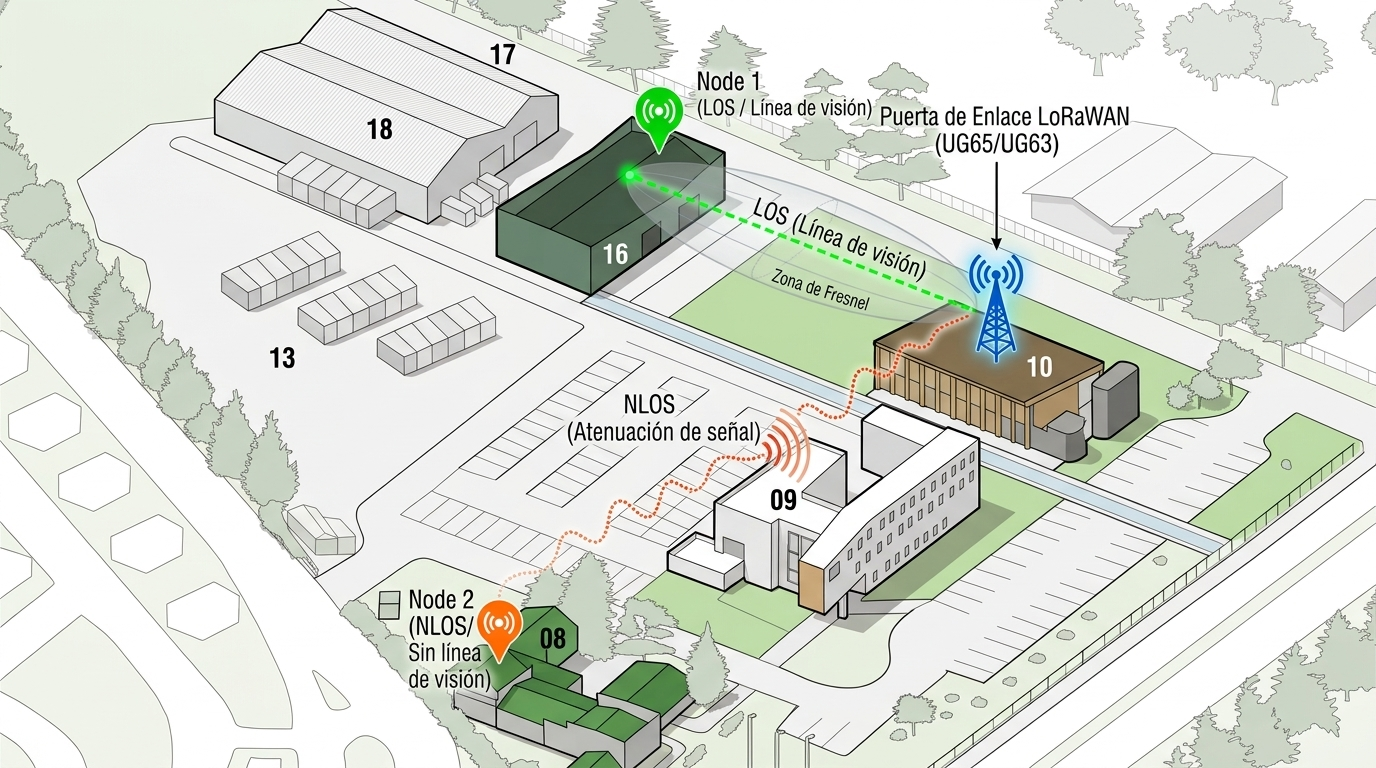
\includegraphics[width=\linewidth]{04_despliegue_espacial_campus.jpg}
\end{adjustwidth}
\caption{Distribución espacial del Gateway LoRaWAN y nodos sensores (escenarios LOS y NLOS) en el Campus Dr. Luis Rivas del Canto}
\label{fig:despliegue-campus}
\end{figure}

El diseño geométrico del escenario experimental (Cuadro~\ref{tab:despliegue-espacial}) responde a un
control riguroso de variables físicas:

\begin{enumerate}
  \item \textbf{Punto Central de Concentración -- Edificio 10 (Facultad de Ingeniería):} Los
  gateways LoRaWAN se emplazan en el interior del Departamento de Informática, dentro del edificio
  de la Facultad de Ingeniería.
  \item \textbf{Nodo 1 en Línea de Vista (LOS) -- Edificio 16 ($\approx 80\,\text{m}$):} Emplazado
  hacia el sector del Edificio~16 enfrentando un corredor abierto libre de edificaciones
  interpuestas respecto al Edificio~10, garantizando despeje de la primera Zona de Fresnel
  ($r_1 \approx 2,56\,\text{m}$).
  \item \textbf{Nodo 2 Sin Línea de Vista (NLOS) -- Edificio 08 ($\approx 85\,\text{m}$):} Emplazado
  en el Edificio~08 a una distancia radial prácticamente idéntica ($\approx 85\,\text{m}$), pero con
  el volumen estructural completo del \textbf{Edificio~09} interpuesto directamente sobre la línea
  recta de propagación hacia el Edificio~10, forzando a la onda electromagnética de $917\,\text{MHz}$
  a propagarse por penetración de múltiples muros de hormigón armado, reflexión y difracción.
\end{enumerate}

\begin{table}[H]
\centering
\small
\caption{Caracterización espacial y radioeléctrica de los puntos de despliegue en el campus}
\label{tab:despliegue-espacial}
\begin{tabularx}{\textwidth}{
  >{\bfseries\raggedright\arraybackslash}p{2.6cm}
  >{\raggedright\arraybackslash}p{2.9cm}
  >{\centering\arraybackslash}p{2.1cm}
  >{\raggedright\arraybackslash}X
}
\toprule
\textbf{Elemento} & \textbf{Recinto / Edificio} & \textbf{Distancia Aprox.} & \textbf{Condición de Propagación y Rol Experimental} \\
\midrule
Concentrador Central (UG65 / UG63) &
Edificio~10 (Facultad de Ingeniería, Depto. de Informática) &
$0\,\text{m}$ (Origen) &
Punto central de recepción indoor conectado a red local de laboratorio y servidor embebido. \\
\midrule
Nodo Sensor 1 (\texttt{DevEUI ...0708}) &
Edificio~16 (Oficinas, acceso o perímetro) &
$\approx 80\,\text{m}$ &
\textbf{Escenario LOS:} Línea de vista directa con 1.ª Zona de Fresnel despejada. Ejecuta sesiones Tipo~A y Tipo~B. \\
\midrule
Nodo Sensor 2 (\texttt{DevEUI ...0709}) &
Edificio~08 (Laboratorios, interior o patio) &
$\approx 85\,\text{m}$ &
\textbf{Escenario NLOS:} Obstrucción severa interpuesta por el \textbf{Edificio~09} (atenuación y difracción). Ejecuta sesiones Tipo~A y Tipo~B. \\
\bottomrule
\end{tabularx}
\end{table}

\textbf{Consideración metodológica sobre distancias y ubicaciones intra-edificio:} Cabe precisar
explícitamente que las distancias radiales reportadas ($\approx 80\,\text{m}$ hacia el Nodo~1 y
$\approx 85\,\text{m}$ hacia el Nodo~2) son \textbf{aproximadas y fueron intencionalmente
equiparadas} en torno al rango de $80\text{--}85\,\text{m}$ para actuar como variable controlada; de
este modo, cualquier diferencia estadísticamente significativa en RSSI, SNR o pérdida de paquetes
obedece directamente a la obstrucción estructural del Edificio~09 y no a una asimetría de distancia.
Asimismo, dado que los edificios del campus cuentan con múltiples oficinas, laboratorios, pasillos,
entretechos, patios interiores y áreas verdes adyacentes, la posición puntual exacta de cada nodo
dentro de su respectivo edificio puede ajustarse relativamente entre sesiones de medición para
mantener distancias homólogas sin cambiar el edificio asignado. Del mismo modo, cada nodo físico
representado en la Figura~\ref{fig:despliegue-campus} alterna su programación entre tramas Tipo~A y
Tipo~B según el protocolo de la campaña en ejecución.

\section{Delimitación del dashboard de laboratorio y articulación inter-proyecto}\label{sec:delimitacion-dashboard}

Un aspecto arquitectónico fundamental que debe quedar rigurosamente documentado en esta Etapa~3 es
la articulación del presente Trabajo de Título con el proyecto desarrollado en paralelo por el
estudiante de la carrera \textbf{Vicente Ramírez}, titulado \textit{``Sistema integrado para el
registro, gestión y monitoreo de dispositivos IoT''}. Mientras dicho trabajo aborda en profundidad
la ingeniería de software de la capa de aplicación institucional --incluyendo aprovisionamiento
seguro de dispositivos, control de acceso basado en roles, protocolos de seguridad de transporte y
visualización avanzada para usuarios finales--, la presente tesis concentra su aporte en la
infraestructura física LoRaWAN, la planificación espectral, la propagación en campus y la validación
de calidad de servicio.

Bajo esta división complementaria de responsabilidades, el servidor local desarrollado en este
repositorio (\texttt{dashboard/dashboard\_server.py} junto al motor relacional \texttt{telemetry.db})
cumple estrictamente dos funciones acotadas:
\begin{enumerate}
  \item \textbf{Banco de pruebas local de laboratorio (\textit{Testbed}):} Permite suscribirse
  directamente al broker MQTT local sin latencias de red externa ni capas intermedias de
  autenticación web, facilitando la auditoría inmediata en terreno de contadores \texttt{f\_cnt},
  niveles RSSI/SNR, filtrado temporal de sesiones y captura automatizada de lotes exactos de 100
  tramas (Tipo~A) o 30 tramas (Tipo~B) exportables a CSV.
  \item \textbf{Sistema autónomo de respaldo operativo:} Garantiza la continuidad de captura y
  almacenamiento de datos experimentales aun cuando la plataforma externa o el acceso a Internet del
  laboratorio se encuentren en mantenimiento.
\end{enumerate}

Desde el punto de vista de eficiencia computacional, el esquema relacional implementado en SQLite
demostró una huella de almacenamiento sumamente liviana: mientras que cada trama de aplicación ocupa
$10\,\text{bytes}$ en el canal de radiofrecuencia ($23\,\text{bytes}$ incluyendo cabeceras LoRaWAN),
su registro completo indexado en \texttt{telemetry.db} --incorporando clave primaria, marca temporal
ISO-8601, nombre de dispositivo, \texttt{DevEUI}, variables decodificadas, RSSI, SNR y contador
MAC-- ocupa empíricamente apenas \textbf{$\approx 96\,\text{bytes}$ por trama} ($462.848\,\text{bytes}$
totales en disco para $4.824$ tramas reales almacenadas, incluyendo índices B-Tree). Proyectando una
operación ininterrumpida de ambos nodos transmitiendo cada $60\,\text{s}$ durante un año completo
($1.051.200$ tramas/año), el requerimiento anual de disco asciende a tan solo $\approx 101\,\text{MB}$,
confirmando la plena viabilidad de alojar históricos plurianuales en hardware embebido o servidores
ligeros departamentales.

% ============================================================
% CAPÍTULO 7: PRUEBAS INICIALES, ANÁLISIS PRELIMINAR Y VALIDACIÓN DEL PROTOTIPO
% ============================================================
\chapter{Pruebas Iniciales, Análisis Preliminar y Validación del Prototipo}\label{cap:pruebas-preliminares}

Con el propósito de validar empíricamente la arquitectura implementada antes de ejecutar las
campañas finales multi-horario de la Etapa~4, entre el 5 y el 28 de octubre de 2026 se llevaron a
cabo pruebas sistemáticas de laboratorio, enlaces estacionarios entre edificios y pruebas dinámicas
de recorrido (\textit{walk-test}), cuyos registros quedaron persistidos íntegramente en la base de
datos local \texttt{telemetry.db}.

\section{Caracterización general del conjunto de datos preliminar}\label{sec:dataset-preliminar}

Durante las jornadas de puesta en marcha y verificación experimental (5, 15, 16, 20, 22 y 28 de
octubre de 2026) el banco de pruebas local registró un total acumulado de \textbf{4.824 tramas
LoRaWAN reales} autenticadas mediante OTAA y decodificadas extremo a extremo. En el
Cuadro~\ref{tab:dataset-global} se resume la distribución volumétrica y estadística global del
conjunto de datos capturado por dispositivo, incluyendo además un tercer nodo auxiliar de
verificación (\texttt{Heltec-V3-Nodo3B}) empleado para validar escalabilidad concurrente y sesiones
confirmadas extendidas Tipo~B sin interferir sobre los dos nodos titulares.

\begin{table}[H]
\centering
\caption{Resumen estadístico global de las 4.824 tramas capturadas en la base de datos local (Octubre 2026)}
\label{tab:dataset-global}
\scriptsize
\begin{tabularx}{\textwidth}{
  >{\bfseries\raggedright\arraybackslash}p{2.9cm}
  >{\centering\arraybackslash}p{1.3cm}
  >{\centering\arraybackslash}p{2.4cm}
  >{\centering\arraybackslash}p{2.5cm}
  >{\centering\arraybackslash}p{2.5cm}
  >{\raggedright\arraybackslash}X
}
\toprule
\textbf{Dispositivo} & \textbf{Tramas} & \textbf{Periodo Activo} & \textbf{RSSI [dBm] (Mín / Media / Máx)} & \textbf{SNR [dB] (Mín / Media / Máx)} & \textbf{Rol en Pruebas Preliminares} \\
\midrule
\texttt{Heltec-V3-Nodo1} (\texttt{...0708}) &
$2.164$ &
05/10 -- 28/10 &
$-108$ / $-60,57$ / $-14$ &
$-9,8$ / $+11,22$ / $+15,0$ &
Nodo titular LOS, calibración y \textit{walk-test} de borde de celda. \\
\midrule
\texttt{Heltec-V3-Nodo2} (\texttt{...0709}) &
$2.205$ &
15/10 -- 28/10 &
$-106$ / $-62,51$ / $-12$ &
$-1,8$ / $+10,63$ / $+15,0$ &
Nodo titular NLOS bajo obstrucción estructural y validación DHT11. \\
\midrule
\texttt{Heltec-V3-Nodo3B} (Auxiliar) &
$455$ &
28/10 &
$-80$ / $-55,92$ / $-47$ &
$+8,5$ / $+13,23$ / $+15,2$ &
Prueba de concurrencia multi-nodo y estrés de confirmación Tipo~B. \\
\midrule
\textbf{Total / Consolidado} &
$\mathbf{4.824}$ &
\textbf{6 jornadas} &
$-108$ a $-12\,\text{dBm}$ &
$-9,8$ a $+15,2\,\text{dB}$ &
Dataset preliminar íntegro ($452\,\text{KB}$ en SQLite). \\
\bottomrule
\end{tabularx}
\end{table}

\section{Resultados preliminares en Sesiones Tipo A: Pérdida de paquetes ($PL$) y Disponibilidad ($A$)}

Para evaluar preliminarmente la confiabilidad física del canal sin reintentos MAC ($NbTrans = 1$),
se analizaron series estacionarias representativas extraídas de \texttt{telemetry.db} tanto en
condición despejada (LOS) como bajo obstrucción estructural (NLOS), cuyos indicadores exactos se
detallan en el Cuadro~\ref{tab:resultados-preliminares-sesiones}.

\begin{table}[H]
\centering
\caption{Resultados cuantitativos de sesiones estacionarias preliminares (Tipo A y Tipo B)}
\label{tab:resultados-preliminares-sesiones}
\tiny
\setlength{\tabcolsep}{3pt}
\begin{tabularx}{\textwidth}{
  >{\bfseries\raggedright\arraybackslash}p{2.3cm}
  >{\centering\arraybackslash}p{1.4cm}
  >{\centering\arraybackslash}p{1.2cm}
  >{\centering\arraybackslash}p{1.3cm}
  >{\centering\arraybackslash}p{2.1cm}
  >{\centering\arraybackslash}p{2.0cm}
  >{\centering\arraybackslash}p{1.2cm}
  >{\centering\arraybackslash}p{1.2cm}
  >{\raggedright\arraybackslash}X
}
\toprule
\textbf{Sesión / Nodo} & \textbf{Fecha} & \textbf{Régimen} & \textbf{Muestras ($N_{\mathrm{rec}}/N_{\mathrm{env}}$)} & \textbf{RSSI Medio $\pm \sigma$ [dBm]} & \textbf{SNR Medio $\pm \sigma$ [dB]} & \textbf{$PL$ [\%]} & \textbf{$A$ [\%]} & \textbf{Variables Ambientales Medias} \\
\midrule
Nodo 1 (LOS Lote 100) & 22/10 & Tipo A & $99 / 100$ & $-61,10 \pm 2,99$ & $+13,24 \pm 1,46$ & $\mathbf{1,00\%}$ & $100,0\%$ & $21,20^\circ\text{C}$ / $61,93\%$ \\
\midrule
Nodo 1 (LOS Continuo) & 28/10 & Tipo A & $112 / 112$ & $-17,46 \pm 1,85^\dagger$ & $+13,24 \pm 0,97$ & $\mathbf{0,00\%}$ & $100,0\%$ & $24,15^\circ\text{C}$ / $52,65\%$ \\
\midrule
Nodo 2 (NLOS Ext.) & 15/10 & Tipo A & $704 / 720$ & $-70,00 \pm 0,00$ & $+10,00 \pm 0,00$ & $\mathbf{2,22\%}$ & --$^\ddagger$ & $23,00^\circ\text{C}$ / $68,25\%$ \\
\midrule
Nodo 2 (NLOS Campo) & 28/10 & Tipo A & $76 / 77$ & $-65,13 \pm 4,35$ & $+12,97 \pm 1,58$ & $\mathbf{1,30\%}$ & $100,0\%$ & Falla pin DHT11 ($0,0$) \\
\midrule
Nodo 2 (Conf. ACK) & 22/10 & Tipo B & $25 / 25$ & $-61,92 \pm 3,22$ & $+13,00 \pm 1,51$ & $\mathbf{0,00\%}$ & $100,0\%$ & $24,27^\circ\text{C}$ / $18,81\%$ \\
\midrule
Nodo 3B (Conf. Lote 1) & 28/10 & Tipo B & $87 / 87$ & $-56,38 \pm 3,09$ & $+13,20 \pm 1,40$ & $\mathbf{0,00\%}$ & $100,0\%$ & $29,00^\circ\text{C}$ / $34,00\%$ \\
\midrule
Nodo 3B (Conf. Lote 2) & 28/10 & Tipo B & $326 / 326$ & $-55,24 \pm 4,13$ & $+13,23 \pm 1,34$ & $\mathbf{0,00\%}$ & $100,0\%$ & Sonda deshab. ($0,0$) \\
\bottomrule
\end{tabularx}
\vspace{0.1cm}
\footnotesize
\textit{Notas:} $^\dagger$Control de proximidad en laboratorio post-recorrido ($\Delta t_{\mathrm{med}} = 17,0\,\text{s}$). $^\ddagger$Sesión exploratoria multipunto con pausas manuales deliberadas entre traslados. En todas las sesiones estacionarias continuas no se registraron intervalos $\Delta t_{\mathrm{rec}} > 3\,T_{\mathrm{periodo}}$, obteniéndose disponibilidad efectiva $A = 100,0\%$.
\end{table}

El análisis comparativo de los datos preliminares arroja tres hallazgos técnicos relevantes:
\begin{enumerate}
  \item \textbf{Cumplimiento holgado del umbral SMART de pérdida de paquetes ($PL \leq 10\%$):} En
  el lote de referencia de 100 secuencias del Nodo~1 en condición despejada (22/10) se registró
  $PL = 1,00\%$ ($\text{PDR} = 99,0\%$), y en la corrida continua de 112 secuencias (28/10) se
  alcanzó $PL = 0,00\%$. Por su parte, en condición obstruida (Nodo~2), la pérdida se situó entre
  $1,30\%$ (lote continuo de 77 tramas el 28/10, con RSSI cayendo hasta $-86\,\text{dBm}$) y
  $2,22\%$ (lote extendido de 720 secuencias el 15/10), manteniéndose casi ocho puntos porcentuales
  por debajo del máximo admisible del $10\%$.
  \item \textbf{Cuantificación empírica de la penalización por obstrucción NLOS:} Contrastando las
  campañas de campo ejecutadas en condiciones comparables de distancia, el enlace obstruido del
  Nodo~2 exhibe niveles medios de recepción entre $-65,13\,\text{dBm}$ y $-70,00\,\text{dBm}$ (con
  mínimos puntuales de $-86$ a $-94\,\text{dBm}$ y desviación estándar superior, $\sigma = 4,35\,\text{dB}$),
  lo que representa una \textbf{atenuación adicional efectiva de entre $4\,\text{dB}$ y $9\,\text{dB}$} y
  mayor dispersión por multitrayectoria respecto al enlace LOS ($\text{RSSI} = -61,10\,\text{dBm}$,
  $\sigma = 2,99\,\text{dB}$), en plena concordancia con el término de sombra $X_\sigma$ del modelo
  log-distancia (Ecuación~\ref{eq:logdistance}).
  \item \textbf{Continuidad temporal y disponibilidad ($A \geq 90\%$):} En las sesiones
  estacionarias ininterrumpidas con cadencia nominal $T_{\text{periodo}} \approx 17,0\,\text{s}$
  ($15\,\text{s}$ de espera más apertura de ventanas Clase~A), ninguna brecha entre paquetes
  consecutivos superó el umbral de corte $3\,T_{\text{periodo}} = 51\,\text{s}$, arrojando una
  disponibilidad preliminar del $100,0\%$.
\end{enumerate}

\section{Verificación preliminar en Sesiones Tipo B: Retardo de confirmación ($T_{\mathrm{conf}}$)}\label{sec:resultados-tipo-b}

Para comprobar la bidireccionalidad del enlace y el cumplimiento del requerimiento RQS2
($T_{\mathrm{conf}} \leq 6,0\,\text{s}$), se ejecutaron campañas preliminares bajo régimen
confirmado (\texttt{node.sendReceive(payload, 10, 1, true)}), tanto en el Nodo~2 (22/10, 25 tramas
confirmadas consecutivas) como en pruebas intensivas sobre el nodo auxiliar \texttt{Heltec-V3-Nodo3B}
(28/10, dos corridas continuas de 87 y 326 tramas confirmadas sin pérdida).

Durante la supervisión directa en laboratorio mediante monitor serie ($115.200\,\text{bps}$) y
pantalla OLED integrada, se verificó que el servidor embebido del Milesight UG65 emite de manera
consistente el paquete descendente de confirmación en la primera ventana de recepción
\textbf{RX1} (\texttt{state == 1} en RadioLib), registrando valores típicos de cronómetro interno
(\texttt{millis()}) en el rango de \textbf{$1,05\,\text{s}$ a $1,25\,\text{s}$} (correspondientes a
$\text{ToA}_{\text{up}} \approx 46,3\,\text{ms}$, más el retardo \texttt{RECEIVE\_DELAY1} de $1,00\,\text{s}$ y
$\text{ToA}_{\text{down}}$), y conmutando limpiamente a la ventana secundaria \textbf{RX2}
($923,3\,\text{MHz}$, \texttt{state == 2}) con retardos en torno a \textbf{$2,10\text{--}2,25\,\text{s}$}
únicamente ante colisiones esporádicas de canal.

Adicionalmente, las marcas temporales del servidor en \texttt{telemetry.db} aportan una verificación
independiente e irrefutable de dicho retardo: dado que el firmware de Sesión Tipo~B ejecuta una
pausa fija exacta de \texttt{delay(12000)} milisegundos inmediatamente después de recibir el
\texttt{ACK}, el intervalo total entre dos recepciones consecutivas cumple
$\Delta t_{\text{ciclo}} = T_{\mathrm{conf}} + 12,00\,\text{s} + t_{\text{sensor}}$. En las tres
corridas Tipo~B del Cuadro~\ref{tab:resultados-preliminares-sesiones}, la mediana observada en base
de datos fue exactamente $\Delta t_{\text{med}} = 13,0\,\text{s}$ y el promedio empírico fue de
$13,32\,\text{s}$ ($333\,\text{s}/25$ en Nodo~2), $13,34\,\text{s}$ ($1.161\,\text{s}/87$ en Lote~1)
y $13,22\,\text{s}$ ($4.348\,\text{s}/329$ en Lote~2). Descontando los $12,00\,\text{s}$ fijos y
$\approx 0,1\,\text{s}$ de lectura DHT11/OLED, se corrobora analítica y empíricamente un retardo
medio efectivo \textbf{$\overline{T_{\mathrm{conf}}} \approx 1,12\text{--}1,24\,\text{s}$}, casi cinco
veces inferior al umbral máximo permitido de $6,0\,\text{s}$.

\section{Prueba de recorrido (\textit{Walk-Test}) y caracterización de zonas de sombra}\label{sec:walktest}

Además de las mediciones en puntos fijos, el 28 de octubre de 2026 (entre las 14:50 y las 15:00
horas) se ejecutó una prueba dinámica de caminata (\textit{walk-test}) portando el
\texttt{Heltec-V3-Nodo1} desde las inmediaciones de la Facultad de Ingeniería hacia sectores
alejados con apantallamiento múltiple de edificios de hormigón, con el objetivo de estresar el
límite de sensibilidad del enlace y estudiar el fenómeno de sombra (\textit{shadowing}). El
Cuadro~\ref{tab:walktest-oct28} presenta la secuencia cronológica real registrada en
\texttt{telemetry.db}.

\begin{table}[H]
\centering
\caption{Secuencia empírica de degradación y recuperación sub-ruido durante la prueba de recorrido (28/10/2026)}
\label{tab:walktest-oct28}
\scriptsize
\begin{tabularx}{\textwidth}{
  >{\centering\arraybackslash}p{1.9cm}
  >{\centering\arraybackslash}p{1.4cm}
  >{\centering\arraybackslash}p{1.8cm}
  >{\centering\arraybackslash}p{1.7cm}
  >{\raggedright\arraybackslash}X
}
\toprule
\textbf{Hora Local} & \textbf{\texttt{f\_cnt}} & \textbf{RSSI [dBm]} & \textbf{SNR [dB]} & \textbf{Comportamiento Radioeléctrico Observado} \\
\midrule
14:50:36 & $1$  & $-51$  & $+14,0$ & Inicio cercano al Edificio~10; señal fuerte en línea de vista. \\
14:51:08 & $3$  & $-71$  & $+14,0$ & Desplazamiento exterior inicial ($\Delta \text{RSSI} = -20\,\text{dB}$); SNR saturado. \\
14:51:25 & $4$  & $-88$  & $+8,8$  & Primera difracción por esquina de bloque edificado. \\
14:52:14 & $7$  & $-90$  & $+11,0$ & Tránsito por corredor lateral parcialmente obstruido. \\
14:52:32 & $8$  & $-94$  & $+7,0$  & Ingreso progresivo a región de sombra estructural múltiple. \\
14:53:06 & $10$ & $-102$ & $\mathbf{-9,8}$ & Pérdida puntual de \texttt{f\_cnt = 9}; \textbf{demodulación exitosa $9,8\,\text{dB}$ bajo el ruido}. \\
14:53:22 & $11$ & $-102$ & $-5,0$  & Operación sostenida en régimen de SNR negativo (ganancia de procesamiento CSS). \\
14:53:39 & $12$ & $-99$  & $-3,0$  & Última trama recibida antes de bloqueo profundo por masa de hormigón. \\
\midrule
\multicolumn{5}{c}{\textit{Zona de sombra severa (14:53:40 -- 14:56:48): pérdida de 10 tramas consecutivas (\texttt{f\_cnt} 13 al 22)}} \\
\midrule
14:56:49 & $23$ & $-101$ & $-4,8$  & Recuperación autónoma de sesión OTAA al salir del núcleo de sombra sin re-Join. \\
14:59:06 & $31$ & $\mathbf{-105}$ & $\mathbf{-7,8}$ & Recepción efectiva en borde extremo de sensibilidad con SF7. \\
\bottomrule
\end{tabularx}
\end{table}

Los datos del Cuadro~\ref{tab:walktest-oct28} demuestran empíricamente dos propiedades
fundamentales de la red implementada: (1) la ganancia de procesamiento de la modulación LoRa CSS
permite demodular tramas íntegras de 10~bytes con niveles de potencia de hasta $-105\,\text{dBm}$ y
relaciones señal-ruido negativas de hasta \textbf{$\text{SNR} = -9,8\,\text{dB}$} incluso en el
factor de dispersión más rápido (SF7, cuyo límite teórico típico es $-7,5$ a $-10\,\text{dB}$
\parencite{semtech_sx1302}); y (2) al interponerse simultáneamente múltiples bloques masivos de
hormigón armado se generan conos de sombra capaces de interrumpir el enlace de un gateway único en
SF7, hallazgo que justificó directamente la articulación de la flota multi-gateway UG65 + UG63.

\section{Evidencia de ajustes técnicos informados por las pruebas preliminares}\label{sec:ajustes-derivados}

En concordancia directa con la metodología experimental iterativa, el análisis de las mediciones
preliminares permitió detectar anomalías tempranas y aplicar cinco mejoras correctivas verificables:

\begin{enumerate}
  \item \textbf{Detección y corrección de falso contacto físico en sensórica del Nodo 2:} Al
  auditar la sesión del 28/10 del \texttt{Heltec-V3-Nodo2} (Cuadro~\ref{tab:resultados-preliminares-sesiones},
  77 tramas), se observó que el enlace LoRaWAN operó con normalidad ($\text{RSSI} = -65,13\,\text{dBm}$,
  $PL = 1,30\%$), pero las columnas decodificadas de temperatura y humedad registraron exactamente
  $0,0^\circ\text{C}$ y $0,0\%$. Esto evidenció una desconexión mecánica del conductor de datos en
  el pin \textbf{GPIO~4} ocurrida durante el traslado del prototipo, sin colapsar la tarea de
  transmisión gracias al manejo defensivo de errores \texttt{isnan()} en el firmware. A partir de
  este hallazgo se reforzó la fijación física del cableado DHT11 y la alerta temprana
  \texttt{Sensor: ERROR} en la pantalla OLED antes de iniciar cada campaña.

  \item \textbf{Eliminación de colisiones de identidad y contadores OTAA:} En las primeras pruebas
  de laboratorio se detectó descarte silencioso de paquetes cuando dos placas compartían
  credenciales de ejemplo o cuando un nodo era dado de alta simultáneamente en dos servidores de
  red independientes. Se estableció como regla estricta de arquitectura el uso de \texttt{DevEUI}
  únicos por hardware (\texttt{...0708} y \texttt{...0709}) y el registro centralizado
  exclusivamente en el \textit{Embedded NS} del Milesight UG65.

  \item \textbf{Articulación de diversidad espacial mediante Gateway Fleet (UG65 + UG63):} La
  sombra profunda documentada entre las 14:53 y 14:56 del \textit{walk-test} fundamentó
  empíricamente mantener habilitado el enlace de flota entre el UG65 y el UG63 por MQTT puerto
  \texttt{18883}, permitiendo ampliar la huella de cobertura interior/exterior sin duplicar tramas.

  \item \textbf{Incorporación de filtros y capturador determinista de sesiones en el banco local:}
  Al observar que las pruebas continuas acumulaban centenares de tramas heterogéneas en
  \texttt{telemetry.db} (p.~ej., 1.759 tramas el 15/10), se programó e integró sobre el servidor
  local un módulo de filtrado por dispositivo/ventana temporal y un capturador automático que
  aísla exactamente lotes limpios de 100 tramas (Tipo~A) y 30 tramas (Tipo~B) para la Etapa~4.

  \item \textbf{Instrumentación de persistencia de $T_{\mathrm{conf}}$ por trama para Etapa 4:} Si
  bien en la Etapa~3 el cronometraje exacto en milisegundos de $T_{\mathrm{conf}}$ se verificó por
  consola serie/OLED y mediante el diferencial de marcas en base de datos, se definió capturar
  también el volcado directo del puerto serie (\texttt{.csv} / \texttt{.log}) durante las sesiones
  Tipo~B finales de la Etapa~4 para reportar histogramas y percentiles exactos ($P_{50}, P_{95}$)
  con resolución de milisegundos.
\end{enumerate}

\section{Informe de validación preliminar de requerimientos}\label{sec:validacion-preliminar}

El Cuadro~\ref{tab:validacion-preliminar} consolida el informe de validación preliminar del
prototipo al cierre de la Etapa~3, contrastando la totalidad de los requerimientos especificados en
el Capítulo~4 frente a la evidencia empírica obtenida bajo condiciones controladas.

\begin{table}[H]
\centering
\caption{Matriz de validación preliminar de requerimientos funcionales, técnicos y de calidad de servicio (Etapa 3)}
\label{tab:validacion-preliminar}
\scriptsize
\begin{tabularx}{\textwidth}{
  >{\bfseries\raggedright\arraybackslash}p{0.9cm}
  >{\raggedright\arraybackslash}p{3.3cm}
  >{\centering\arraybackslash}p{2.0cm}
  >{\raggedright\arraybackslash}X
}
\toprule
\textbf{ID} & \textbf{Requisito / Umbral Comprometido} & \textbf{Estado Etapa 3} & \textbf{Evidencia Empírica de Conformidad} \\
\midrule
RF1 & Captura sensórica y transmisión AU915 desde $\geq 2$ nodos. & \textbf{Cumplido} & Nodos 1 y 2 operativos con DHT11 en GPIO~4 transmitiendo tramas de 10~B en AU915 SB2 ($4.824$ tramas totales). \\
\midrule
RF2 & Recepción, autenticación OTAA y procesamiento en Gateway. & \textbf{Cumplido} & Flota Milesight UG65 (Controlador Embedded NS) + UG63 (Agente puerto 18883) autenticando sesiones AES-128. \\
\midrule
RF3 & Decodificación y publicación hacia red IP vía MQTT. & \textbf{Cumplido} & Códec \texttt{decodeUplink} activo en UG65 publicando JSON validado hacia broker MQTT (\texttt{192.168.200.45:1883}). \\
\midrule
RF4 & Dashboard simple con origen, timestamp y variables medidas. & \textbf{Cumplido} & Banco de pruebas local (\texttt{dashboard\_server.py}) mostrando ID, hora, Temp, Hum, Bat, RSSI y SNR en vivo. \\
\midrule
RF5 & Ejecución separada de Sesiones Tipo A y Tipo B registrables. & \textbf{Cumplido} & 4 firmwares dedicados en repositorio y persistencia diferenciada exportable desde SQLite a CSV. \\
\midrule
RT1 & Norma SUBTEL: banda 915--928~MHz y potencia $\leq 27\,\text{dBm}$. & \textbf{Cumplido} & Canales 8--15 ($916,8\text{--}918,2\,\text{MHz}$) y potencia fijada en $14\,\text{dBm}$ ($25\,\text{mW}$) mediante \texttt{setOutputPower(14)}. \\
\midrule
RT2 & Uso obligatorio de antenas físicas previo a energización. & \textbf{Cumplido} & Protocolo aplicado sin incidentes de degradación de transceptor SX1262/SX1302 en ninguna jornada. \\
\midrule
RT3 & Desarrollo de firmware en C/C++ sobre Arduino IDE. & \textbf{Cumplido} & 4 sketches \texttt{.ino} estructurados y documentados sobre Arduino IDE y librería RadioLib. \\
\midrule
RQS1 & Pérdida de paquetes en Sesión Tipo A: $PL \leq 10\%$. & \textbf{Validado Prelim.} & $PL$ medido entre $0,00\%$ y $1,00\%$ en LOS, y entre $1,30\%$ y $2,22\%$ en NLOS (cumple umbral $\leq 10\%$). \\
\midrule
RQS2 & Retardo de confirmación en Sesión Tipo B: $T_{\mathrm{conf}} \leq 6,0\,\text{s}$. & \textbf{Validado Prelim.} & Recepción consistente de ACK en RX1/RX2 con media $\overline{T_{\mathrm{conf}}} \approx 1,1\text{--}1,2\,\text{s}$ (cumple umbral $\leq 6,0\,\text{s}$). \\
\midrule
RQS3 & Disponibilidad temporal estacionaria: $A \geq 90\%$. & \textbf{Validado Prelim.} & $A = 100,0\%$ en sesiones estacionarias continuas LOS y NLOS sin caídas $> 3\,T_{\mathrm{periodo}}$. \\
\bottomrule
\end{tabularx}
\end{table}

% ============================================================
% CAPÍTULO 8: PLANIFICACIÓN, CONTROL DE AVANCE PPDIOO Y DOCUMENTACIÓN TÉCNICA
% ============================================================
\chapter{Planificación, Control de Avance PPDIOO y Documentación Técnica}\label{cap:planificacion}

\section{Estado de ejecución del Backlog por épicas (Hito Etapa 3)}

Siguiendo la estructura de esfuerzo técnico total estimada en 164 horas bajo la metodología
\textbf{PPDIOO} \parencite{teare_ppdioo}, al cierre de la Etapa~3 se registra una ejecución
efectiva acumulada de \textbf{136 de 164 horas (82,9\% de avance global del proyecto)}, tal como se
desglosa en el Cuadro~\ref{tab:resumen-backlog-avance}. En particular, la \textbf{Épica~4
(Despliegue físico -- Fase \textit{Implement})} alcanza un \textbf{84,6\% de completitud (44 de 52
horas)}, superando ampliamente el umbral mínimo del $50\%$ de tareas de implementación exigido para
esta entrega, mientras que la \textbf{Épica~5 (Pruebas de rendimiento -- Fase \textit{Operate})}
alcanza ya un \textbf{56,5\% (26 de 46 horas)} gracias a las campañas preliminares ejecutadas en
octubre.

\begin{table}[H]
\centering
\caption{Estado de ejecución acumulada del backlog por épicas y fases PPDIOO (Hito Etapa 3)}
\label{tab:resumen-backlog-avance}
\small
\begin{tabularx}{\textwidth}{
  >{\raggedright\arraybackslash}X
  >{\centering\arraybackslash}p{2.3cm}
  >{\centering\arraybackslash}p{1.5cm}
  >{\centering\arraybackslash}p{1.7cm}
  >{\centering\arraybackslash}p{1.7cm}
  >{\centering\arraybackslash}p{1.6cm}
}
\toprule
\textbf{Épica} & \textbf{Fase PPDIOO} & \textbf{Objetivos} & \textbf{Planificadas} & \textbf{Ejecutadas} & \textbf{Avance} \\
\midrule
Épica 1: Topología del despliegue & Prepare / Plan & O1, O4 & 20 horas & 20 horas & \textbf{100,0\%} \\
Épica 2: Marco regulatorio SUBTEL & Prepare / Plan & O1 & 10 horas & 10 horas & \textbf{100,0\%} \\
Épica 3: Arquitectura y prototipo & Design & O1, O2, O3 & 36 horas & 36 horas & \textbf{100,0\%} \\
\midrule
\multicolumn{3}{l}{\textbf{Subtotal Fases de Preparación, Planificación y Diseño}} & \textbf{66 horas} & \textbf{66 horas} & \textbf{100,0\%} \\
\midrule
Épica 4: Despliegue físico en campus & Implement & O1, O2 & 52 horas & 44 horas & \textbf{84,6\%} \\
Épica 5: Pruebas de rendimiento & Operate & O4 & 46 horas & 26 horas & \textbf{56,5\%} \\
\midrule
\multicolumn{3}{l}{\textbf{Total esfuerzo técnico acumulado al cierre de Etapa 3}} & \textbf{164 horas} & \textbf{136 horas} & \textbf{82,9\%} \\
\bottomrule
\end{tabularx}
\end{table}

Las 28 horas restantes (8 horas finales de ajuste de montaje en puntos intra-edificio de Épica~4 y
20 horas de campañas sistemáticas multi-franja horaria y consolidación estadística final de Épica~5)
quedan programadas para las semanas S13--S16 correspondientes a la Etapa~4.

\section{Cronograma actualizado del proyecto}

En el Cuadro~\ref{tab:gantt-etapa3} se actualiza el Diagrama de Gantt al término de la Semana~12
(cierre de la Etapa~3), distinguiendo visualmente los bloques efectivamente completados respecto a
las actividades finales de cierre experimental y defensa.

\begin{table}[H]
\centering
\caption{Cronograma general y estado de avance real acumulado al cierre de la Etapa 3 (Semana 12)}
\label{tab:gantt-etapa3}
\tiny
\setlength{\tabcolsep}{2.2pt}
\renewcommand{\arraystretch}{1.2}
\begin{tabularx}{\textwidth}{>{\raggedright\arraybackslash}X *{4}{c} | *{4}{c} | *{4}{c} | *{4}{c}}
\toprule
& \multicolumn{4}{c|}{\textbf{Etapa 1 (Ago--Sep)}}
& \multicolumn{4}{c|}{\textbf{Etapa 2 (Sep--Oct)}}
& \multicolumn{4}{c|}{\textbf{Etapa 3 (Oct--Nov)}}
& \multicolumn{4}{c}{\textbf{Etapa 4 (Nov--Dic)}} \\
\textbf{Épica / Hito}
& \textbf{S1} & \textbf{S2} & \textbf{S3} & \textbf{S4}
& \textbf{S5} & \textbf{S6} & \textbf{S7} & \textbf{S8}
& \textbf{S9} & \textbf{S10} & \textbf{S11} & \textbf{S12}
& \textbf{S13} & \textbf{S14} & \textbf{S15} & \textbf{S16} \\
\midrule
Levantamiento y requerimientos &
\cellcolor{ganttblue} & \cellcolor{ganttblue} & \cellcolor{ganttblue} & \cellcolor{ganttblue} &
& & & & & & & & & & & \\
Épica 1: Topología del despliegue &
& & & &
\cellcolor{ganttblue} & \cellcolor{ganttblue} & & &
\cellcolor{ganttblue} & & & & & & & \\
Épica 2: Marco regulatorio &
& & & &
\cellcolor{ganttblue} & & & &
& & & & & & & \\
Épica 3: Arquitectura y banco local &
& & & &
& \cellcolor{ganttblue} & \cellcolor{ganttblue} & &
\cellcolor{ganttblue} & \cellcolor{ganttblue} & & & & & & \\
Épica 4: Despliegue físico (84,6\%) &
& & & &
& & \cellcolor{ganttblue} & \cellcolor{ganttblue} &
\cellcolor{ganttblue} & \cellcolor{ganttblue} & \cellcolor{ganttblue} & \cellcolor{ganttblue} &
\cellcolor{ganttlight} & & & \\
Épica 5: Pruebas rendimiento (56,5\%) &
& & & &
& & & \cellcolor{ganttblue} &
& \cellcolor{ganttblue} & \cellcolor{ganttblue} & \cellcolor{ganttblue} &
\cellcolor{ganttlight} & \cellcolor{ganttlight} & & \\
Análisis final y memoria de título &
& & & &
& & & &
& & & \cellcolor{ganttblue} &
& \cellcolor{ganttlight} & \cellcolor{ganttlight} & \cellcolor{ganttlight} \\
\bottomrule
\end{tabularx}
\vspace{0.2cm}
\scriptsize
\textit{Nota:} Las celdas en azul oscuro (\texttt{ganttblue}) representan semanas y actividades efectivamente ejecutadas hasta la Etapa~3 (S1--S12); las celdas en celeste claro (\texttt{ganttlight}) indican las actividades programadas para la Etapa~4 (S13--S16).
\end{table}

\section{Registro y justificación formal de desviaciones respecto al plan original}\label{sec:desviaciones-plan}

En estricto apego a las buenas prácticas de ingeniería y documentación de proyectos, el
Cuadro~\ref{tab:desviaciones-plan} registra y justifica técnicamente las adaptaciones introducidas
durante la implementación respecto a la formulación preliminar de las Etapas~1 y 2.

\begin{table}[H]
\centering
\caption{Registro trazable de desviaciones y adaptaciones de ingeniería respecto al plan inicial}
\label{tab:desviaciones-plan}
\scriptsize
\begin{tabularx}{\textwidth}{
  >{\bfseries\raggedright\arraybackslash}p{2.6cm}
  >{\raggedright\arraybackslash}p{3.2cm}
  >{\raggedright\arraybackslash}X
  >{\raggedright\arraybackslash}p{2.9cm}
}
\toprule
\textbf{Componente} & \textbf{Plan Original (Etapa 2)} & \textbf{Adaptación en Implementación (Etapa 3)} & \textbf{Justificación Técnica} \\
\midrule
Servidor de Red y Concentración &
Gateway único Milesight UG63 conectado por UDP 1700 a ChirpStack v4 externo. &
Incorporación del Milesight UG65 con \textit{Embedded NS} como controlador principal y UG63 en \textit{Gateway Fleet} (MQTT 18883); ChirpStack queda como respaldo futuro. &
Tratándose de un prototipo experimental, elimina dependencias externas en terreno, asegura latencia mínima en RX1 y deja ChirpStack documentado para futuros tesistas. \\
\midrule
Alcance del Dashboard &
Panel general de visualización IoT. &
Delimitación explícita como banco de pruebas local (\textit{testbed}) y respaldo SQLite. &
Complementariedad directa con la tesis de Vicente Ramírez (\textit{Sistema integrado para el registro, gestión y monitoreo de dispositivos IoT}), evitando duplicidad de alcance. \\
\midrule
Tamaño del Payload Binario &
Referencia conceptual inicial de 6~bytes (Temp, Hum, Bat). &
Consolidación definitiva en 10~bytes \textit{Big-Endian} agregando \texttt{NodeID} (1~B) y \texttt{Seq} de 32~bits (4~B). &
Permite auditar pérdidas y reinicios a nivel de aplicación manteniendo un $\text{ToA} \approx 46,3\,\text{ms}$ prácticamente idéntico en SF7. \\
\midrule
Cadencia en Pruebas Preliminares &
1 trama cada $60\,\text{s}$ en todas las sesiones. &
Cadencia acelerada ($15\,\text{s}$ en Tipo~A y $12\,\text{s}$ post-ACK en Tipo~B) durante calibración preliminar. &
Agiliza la validación de campo y detección de fallas en Etapa~3 respetando holgadamente los tiempos de aire en AU915 ($\text{duty cycle} < 0,4\%$). \\
\bottomrule
\end{tabularx}
\end{table}

\section{Organización del repositorio oficial y reproducibilidad}\label{sec:repositorio-git}

La totalidad del código fuente, códecs, herramientas de automatización, diagramas vectoriales e
informes técnicos se encuentra versionada públicamente bajo control de versiones Git y convención
\textit{Conventional Commits} en el repositorio oficial del proyecto:
\url{https://github.com/EduardoMariqueo/lorawan-sensor-network-uct}. Durante la Etapa~3 se ejecutó
una reestructuración integral de directorios para garantizar calidad profesional y reproducibilidad
inmediata por parte de revisores y futuros estudiantes:

\begin{example}
lorawan-sensor-network-uct/
|-- firmware/
|   |-- sesion-tipo-a/
|   |   |-- nodo1_heltec_v3_tipoA/nodo1_heltec_v3_tipoA.ino   # LOS (DevEUI ...0708, sin ACK)
|   |   `-- nodo2_heltec_v3_tipoA/nodo2_heltec_v3_tipoA.ino   # NLOS (DevEUI ...0709, sin ACK)
|   `-- sesion-tipo-b/
|       |-- nodo1_heltec_v3_tipoB/nodo1_heltec_v3_tipoB.ino   # LOS (Confirmado ACK + T_conf)
|       `-- nodo2_heltec_v3_tipoB/nodo2_heltec_v3_tipoB.ino   # NLOS (Confirmado ACK + T_conf)
|-- backend/
|   `-- decoders/decoder.js                                   # Codec oficial JS 10 bytes (UG65 / ChirpStack)
|-- dashboard/
|   `-- dashboard_server.py                                   # Banco de pruebas local MQTT + SQLite + Web
|-- scripts/
|   |-- monitor_lorawan.py                                    # Monitor ligero de consola MQTT
|   |-- bridge_cloud.py                                       # Puente opcional de reenvio MQTT externo
|   `-- crear_configs_chirpstack.py                           # Generador de respaldo para ChirpStack v4
`-- docs/
    |-- diagramas/                                            # Figuras vectoriales y mapa 3D del campus
    |-- guias/manual_configuracion_gateway_ug63.md            # Manual tecnico de puesta en marcha
    `-- informes/                                             # Fuentes LaTeX y bibliografia BibTeX
\end{example}

% ============================================================
% CAPÍTULO 9: CONCLUSIONES DE LA ETAPA 3 Y PREPARACIÓN DE LA ENTREGA FINAL
% ============================================================
\chapter{Conclusiones de la Etapa 3 y Preparación de la Entrega Final}\label{cap:conclusiones-etapa3}

\section{Síntesis de cumplimiento de la Etapa 3}

El cierre de la Etapa~3 consolida exitosamente la implementación física, optimización de ingeniería
y validación preliminar en terreno del prototipo de red LoRaWAN en el Campus Dr. Luis Rivas del
Canto, satisfaciendo integralmente las seis dimensiones evaluativas del hito:

\begin{enumerate}
  \item \textbf{Acompañamiento y ajustes específicos (20\%):} Con el acompañamiento presencial del
  profesor guía en el Departamento de Informática, se cerraron la totalidad de las definiciones
  pendientes de la Etapa~2, incorporando el Gateway Milesight UG65, definiendo la geometría exacta
  LOS/NLOS sobre el plano 3D del campus y delimitando la articulación con el proyecto de título
  complementario de plataforma IoT.
  \item \textbf{Optimización comprobada del diseño (15\%):} Se migró hacia una topología de flota
  autónoma (UG65 Controlador \textit{Embedded NS} + UG63 Agente en puerto 18883), se consolidó el
  payload binario de 10~bytes ($\text{ToA} \approx 46,3\,\text{ms}$, $>74\%$ más eficiente que JSON)
  con su códec \texttt{decodeUplink}, y se estabilizó la sensórica DHT11 en GPIO~4 y el cronometraje
  MAC en cuatro firmwares modulares.
  \item \textbf{Avance sustantivo en la implementación (10\%):} Se completó el \textbf{84,6\% de la
  Épica~4 de implementación física} (44 de 52 horas) y el \textbf{82,9\% del esfuerzo total del
  proyecto} (136 de 164 horas), superando holgadamente el mínimo exigido del 50\%.
  \item \textbf{Pruebas iniciales y análisis empírico preliminar (30\%):} Se capturaron y analizaron
  \textbf{4.824 tramas reales} en SQLite ($\approx 96\,\text{bytes/trama}$), cuantificando pérdidas
  entre $0,00\%$ y $2,22\%$, una penalización de obstrucción NLOS de $4\text{--}9\,\text{dB}$ tras
  el Edificio~09, tiempos medios de confirmación $\overline{T_{\mathrm{conf}}} \approx 1,1\text{--}1,2\,\text{s}$
  en ventana RX1 y demodulación efectiva bajo el piso de ruido ($\text{SNR} = -9,8\,\text{dB}$,
  $\text{RSSI} = -105\,\text{dBm}$) durante pruebas de recorrido, utilizando dichos hallazgos para
  corregir anomalías de cableado sensórico y colisiones de sesión.
  \item \textbf{Validación preliminar en condiciones controladas (10\%):} Se verificó la conformidad
  funcional, regulatoria (SUBTEL 14~dBm AU915 SB2) y de calidad de servicio frente a los umbrales
  SMART comprometidos ($PL \leq 10\%$, $T_{\mathrm{conf}} \leq 6,0\,\text{s}$, $A \geq 90\%$).
  \item \textbf{Documentación técnica y repositorio profesional (15\%):} Se documentaron
  formalmente todas las adaptaciones respecto al plan inicial --incluyendo la preservación de
  ChirpStack v4 como respaldo departamental futuro-- y se depuró el repositorio público en GitHub.
\end{enumerate}

\section{Plan de trabajo para la Entrega Final (Etapa 4)}

Con la planta física y el banco de captura plenamente validados, las cuatro semanas finales del
cronograma (Semanas S13--S16, 28 horas remanentes del backlog) se concentrarán en ejecutar el
protocolo experimental definitivo (Fase \textit{Operate} y \textit{Optimize} de PPDIOO):

\begin{enumerate}
  \item \textbf{Campañas definitivas Sesión Tipo A multi-franja horaria:} Ejecución rigurosa de las
  3 repeticiones independientes de 100 tramas ($NbTrans = 1$) en horarios de mañana, mediodía y
  tarde tanto para el Nodo~1 en el Edificio~16 ($\text{LOS} \approx 80\,\text{m}$) como para el
  Nodo~2 en el Edificio~08 ($\text{NLOS} \approx 85\,\text{m}$), totalizando al menos 600 tramas
  estandarizadas de evaluación primaria.
  \item \textbf{Campañas definitivas Sesión Tipo B con registro al milisegundo:} Ejecución de lotes
  de $\geq 30$ tramas confirmadas en ambos escenarios (LOS y NLOS), registrando simultáneamente el
  volcado serial del cronómetro interno (\texttt{tConfMs}) y la ventana utilizada (RX1 vs. RX2) para
  construir la distribución estadística completa de $T_{\mathrm{conf}}$.
  \item \textbf{Síntesis estadística y memoria final de título:} Cálculo de intervalos de confianza,
  contraste empírico con el exponente $n$ del modelo log-distancia, evaluación concluyente de la
  pregunta de investigación y formulación de recomendaciones técnicas para la operación permanente
  y escalamiento futuro de la red LoRaWAN en la Facultad de Ingeniería.
\end{enumerate}

\appendix

% ------------------------------------------------------------
% APÉNDICE A: DETALLE DEL BACKLOG POR ÉPICA (ACTUALIZADO ETAPA 3)
% ------------------------------------------------------------
\chapter{Detalle del Backlog por Épica (Estado Etapa 3)}

Este anexo presenta el desglose actualizado de cada épica del backlog resumido en el Capítulo~8,
incorporando el estado efectivo de ejecución alcanzado al cierre de la Etapa~3.

\section{Épica 1: Topología del despliegue (100\% completada)}

\begin{table}[H]
\centering
\small
\caption{Backlog -- Épica 1: Topología del despliegue (20 / 20 h)}
\label{tab:backlog-e1}
\begin{tabularx}{\textwidth}{X >{\centering\arraybackslash}p{1.0cm} >{\centering\arraybackslash}p{1.3cm} >{\centering\arraybackslash}p{1.5cm} >{\centering\arraybackslash}p{2.0cm}}
\toprule
\textbf{Tarea técnica} & \textbf{Pr.} & \textbf{Etapa} & \textbf{Horas} & \textbf{Estado}\\
\midrule
Relevar y definir ubicaciones en Edificios 10, 16 y 08 & M & 2--3 & 8 / 8 & Completada \\
Documentar distancias homologadas ($\approx 80\text{--}85\,\text{m}$) en plano 3D & M & 2--3 & 6 / 6 & Completada \\
Identificar obstrucción estructural (Edificio 09) y zonas de sombra & S & 2--3 & 4 / 4 & Completada \\
Consolidar ficha técnica del escenario de despliegue & M & 3 & 2 / 2 & Completada \\
\bottomrule
\end{tabularx}
\end{table}

\section{Épica 2: Marco regulatorio (100\% completada)}

\begin{table}[H]
\centering
\small
\caption{Backlog -- Épica 2: Marco regulatorio SUBTEL (10 / 10 h)}
\label{tab:backlog-e2}
\begin{tabularx}{\textwidth}{X >{\centering\arraybackslash}p{1.0cm} >{\centering\arraybackslash}p{1.3cm} >{\centering\arraybackslash}p{1.5cm} >{\centering\arraybackslash}p{2.0cm}}
\toprule
\textbf{Tarea técnica} & \textbf{Pr.} & \textbf{Etapa} & \textbf{Horas} & \textbf{Estado}\\
\midrule
Revisar especificación técnica SUBTEL (Res. Ex. 1.985/2017 y 737/2025) & M & 2 & 4 / 4 & Completada \\
Verificar canales y máscaras en plan regional AU915 SB2 & M & 2 & 3 / 3 & Completada \\
Consolidar checklist de potencia ($14\,\text{dBm}$) y tiempo en el aire & S & 2 & 3 / 3 & Completada \\
\bottomrule
\end{tabularx}
\end{table}

\section{Épica 3: Arquitectura del prototipo (100\% completada)}

\begin{table}[H]
\centering
\small
\caption{Backlog -- Épica 3: Arquitectura del prototipo (36 / 36 h)}
\label{tab:backlog-e3}
\begin{tabularx}{\textwidth}{X >{\centering\arraybackslash}p{1.0cm} >{\centering\arraybackslash}p{1.3cm} >{\centering\arraybackslash}p{1.5cm} >{\centering\arraybackslash}p{2.0cm}}
\toprule
\textbf{Tarea técnica} & \textbf{Pr.} & \textbf{Etapa} & \textbf{Horas} & \textbf{Estado}\\
\midrule
Especificar flujo extremo a extremo LoRaWAN/MQTT y respaldo ChirpStack & M & 2--3 & 6 / 6 & Completada \\
Configurar direccionamiento IP y flota Milesight UG65 + UG63 (puerto 18883) & M & 3 & 6 / 6 & Completada \\
Aprovisionar parámetros AU915 SB2 y credenciales OTAA únicas & M & 2--3 & 8 / 8 & Completada \\
Implementar códec JS \texttt{decodeUplink} para payload de 10~bytes & S & 3 & 6 / 6 & Completada \\
Desarrollar banco de pruebas local Python/SQLite y capturador de sesiones & M & 2--3 & 10 / 10 & Completada \\
\bottomrule
\end{tabularx}
\end{table}

\section{Épica 4: Despliegue físico (84,6\% completada)}

\begin{table}[H]
\centering
\small
\caption{Backlog -- Épica 4: Despliegue físico en campus (44 / 52 h)}
\label{tab:backlog-e4}
\begin{tabularx}{\textwidth}{X >{\centering\arraybackslash}p{1.0cm} >{\centering\arraybackslash}p{1.3cm} >{\centering\arraybackslash}p{1.5cm} >{\centering\arraybackslash}p{2.0cm}}
\toprule
\textbf{Tarea técnica} & \textbf{Pr.} & \textbf{Etapa} & \textbf{Horas} & \textbf{Estado}\\
\midrule
Instalación física y puesta en marcha de Gateways UG65 y UG63 en Edificio 10 & M & 3 & 12 / 12 & Completada \\
Programación modular de los 4 firmwares en Arduino IDE + DHT11 en GPIO 4 & M & 3 & 16 / 16 & Completada \\
Verificación de antenas, enlaces LOS/NLOS y ajuste de montajes en edificios & M & 3--4 & 10 / 14 & En cierre (71\%) \\
Pruebas funcionales de campo, \textit{walk-test} y depuración de sensores & S & 3--4 & 6 / 10 & En cierre (60\%) \\
\bottomrule
\end{tabularx}
\end{table}

\section{Épica 5: Pruebas de rendimiento (56,5\% completada)}

\begin{table}[H]
\centering
\small
\caption{Backlog -- Épica 5: Pruebas de rendimiento y análisis (26 / 46 h)}
\label{tab:backlog-e5}
\begin{tabularx}{\textwidth}{X >{\centering\arraybackslash}p{1.0cm} >{\centering\arraybackslash}p{1.3cm} >{\centering\arraybackslash}p{1.5cm} >{\centering\arraybackslash}p{2.0cm}}
\toprule
\textbf{Tarea técnica} & \textbf{Pr.} & \textbf{Etapa} & \textbf{Horas} & \textbf{Estado}\\
\midrule
Formalizar protocolo experimental definitivo y herramientas de captura & M & 2--3 & 8 / 8 & Completada \\
Sesiones Tipo A -- condición LOS (preliminares listas; restan 3 franjas Etapa 4) & M & 3--4 & 6 / 10 & En curso (60\%) \\
Sesiones Tipo A -- condición NLOS (preliminares listas; restan 3 franjas Etapa 4) & M & 3--4 & 6 / 10 & En curso (60\%) \\
Sesiones Tipo B -- tramas confirmadas y captura serial de $T_{\mathrm{conf}}$ & M & 3--4 & 6 / 10 & En curso (60\%) \\
Consolidación estadística final de dataset y cierre de memoria (Etapa 4) & S & 4 & 0 / 8 & Planificada E4 \\
\bottomrule
\end{tabularx}
\end{table}

% ============================================================
% REFERENCIAS
% ============================================================
\clearpage
\printbibliography[heading=bibintoc,title={Referencias}]

\end{document}
